\documentclass[a4paper]{article}

\usepackage{NotesPackage2}
\usepackage{listings}
\usepackage{xcolor}
\usepackage{multicol}
\usepackage[vlined, algosection]{algorithm2e}

\author{Willoughby Seago}
\date{September 22, 2020}
\title{Numerical Recipes}

\usetikzlibrary{decorations.markings, decorations.pathreplacing}

\makeglossaries
% Add glossary entries here
\newacronym{dft}{DFT}{discrete Fourier transform}
\newacronym{fft}{FFT}{fast Fourier transform}
\newacronym{ode}{ODE}{ordinary differential equation}
\newacronym{pde}{PDE}{partial differential equation}
\newacronym{ivp}{IVP}{initial value problem}
\newacronym{bvp}{BVP}{boundary value problem}
\newacronym{cpu}{CPU}{central processing unit}
\newacronym{lu}{LU}{lower-upper}
\newacronym{svd}{SVD}{single value decomposition}
\newacronym{le}{LE}{Laplace equation}
\newacronym{bc}{BC}{boundary condition}
\newacronym{rng}{RNG}{random number generator}
\newacronym{lcg}{LCG}{linear congruential generator}
\newacronym{pdf}{PDF}{probability density function}
\newacronym{cdf}{CDF}{cumulative density function}
\newacronym{lpf}{LPF}{low pass filter}
\newacronym{hpf}{HPF}{high pass filter}
\newacronym{mlm}{MLM}{maximum likelihood method}
\newacronym{abc}{ABC}{approximate Bayesian computation}
\newacronym{lhc}{LHC}{large hadron collider}
\newacronym{gpu}{GPU}{graphics processing unit}
\newacronym{cnn}{CNN}{convolutional neural network}
\newacronym{ann}{ANN}{adversarial neural network}

\definecolor{keywordColor}{HTML}{008000}
\definecolor{numberColor}{HTML}{505050}
\definecolor{commentColor}{HTML}{797979}
\definecolor{stringColor}{HTML}{BA2121}

\lstset{
    language=python,
    keywordstyle=\color{keywordColor},
    commentstyle={\itshape\color{commentColor}},
    stringstyle={\ttfamily\color{stringColor}},
    showstringspaces=false,
    numberstyle=\color{numberColor}\tiny,
    numbers=left,
    numbersep=-0.5cm
}

\DontPrintSemicolon  % no semicolons when writing algorithms

\newcommand{\notesVersion}{1.0}
\newcommand{\notesDate}{23/12/2020}
\DeclareMathOperator{\sgn}{sgn}
\newcommand{\st}{\mid}
\newcommand{\FT}{\mathcal{F}}
\newcommand{\convolution}{*}

\includeonly{}

\begin{document}
    \pagenumbering{roman}  % Number contents pages and glossaries with roman numerals
    \maketitle
    These are my notes for the \textit{numerical recipes} course from the University of Edinburgh as part of the third year of the theoretical physics degree.
    When I took this course in the 2020/21 academic year it was taught by Dr Bartlomiej Waclaw\footnote{\url{https://www.ph.ed.ac.uk/people/bartlomiej-waclaw}} and Dr Britton Smith\footnote{\url{https://www.ph.ed.ac.uk/people/britton-smith}}.
    These notes are based on the lectures delivered as part of this course, the notes provided as part of this course, and the book `numerical recipes'\footnote{Press, W.~H. et al. \textit{Numerical Recipes}, third edition (Cambridge University Press, Cambridge, 2007)}.
    The content within is correct to the best of my knowledge but if you find a mistake or just disagree with something or think it could be improved please let me know.
    
    These notes were produced using \LaTeX\footnote{\url{https://www.latex-project.org/}}.
    Graphs where plotted using Matplotlib\footnote{\url{https://matplotlib.org/}}, NumPy\footnote{\url{https://numpy.org/}}, and SciPy\footnote{\url{https://scipy.org/scipylib/}}.
    Diagrams were drawn with tikz\footnote{\url{https://www.ctan.org/pkg/pgf}}.
    Code was written using listings\footnote{\url{https://www.ctan.org/pkg/listings}} and algorithms where written using algorithm2e\footnote{\url{https://www.ctan.org/pkg/algorithm2e}}.
    
    This is version \notesVersion~of these notes, which is up to date as of \notesDate.
    \begin{flushright}
        Willoughby Seago
        
        s1824487@ed.ac.uk
    \end{flushright}
    \clearpage
    \tableofcontents
    \listoffigures
    \listoftables
    \listofalgorithms
    \printglossary[type=\acronymtype, title=Acronyms, style=long]
    \clearpage
    \pagenumbering{arabic}  % Number rest of document with numbers
    \begingroup
    \let\clearpage\relax  % "\begingroup, \let\clearpage\relax, \endgroup" stops automatic pagebreaks after each include
    % \include sections here
    \endgroup
    \section{Algorithms}
    \subsection{Classifying Algorithms}
    We will consider here two different ways to classify algorithms.
    The first refers to the predictability of the out put.
    An algorithm can be
    \begin{itemize}
        \item deterministic -- given a set input the output is always the same,
        \item stochastic -- given a set input the output may change.
    \end{itemize}
    Another way to classify an algorithm is based on the way in which it loops.
    The two most common ways to loop are:
    \begin{itemize}
        \item iteratively -- a loop over some objects such as some numbers, an array, or a string,
        \item recursively -- a function that calls itself.
    \end{itemize}
    An example of a deterministic, iterative, program is
    \begin{lstlisting}[language=python]
    total = 0
    for i in range(1, 100):
        total += 1
    print(total)
    \end{lstlisting}
    This will print 99 every time.
    A slight change to this will make it stochastic instead:
    \begin{lstlisting}[language=python]
    import numpy as np
    total = 0
    for i in range(1, 100):
        total += np.random.unioform(0, 2)
    print(total)
    \end{lstlisting}
    Running this four times gives four different answers: 94.4, 90.6, 109.8, and 97.0, all to 1 decimal place.
    A deterministic, recursive function is given below:
    \begin{lstlisting}[language=python]
    def f(n):
        if n == 1:
            return 1
        return f(n - 1) + 1
    print(f(10))
    \end{lstlisting}
    This will print 10 every time.
    
    \subsection{Types of Numerical Variables}
    \subsubsection{Integers}
    Integers, or \lstinline|int|, in python, as the name suggests, store whole numbers, \(0, \pm 1, \pm 2, \dotsc\).
    In python 3 the \lstinline|int| class supports integers of any size, positive or negative (or zero).
    There are fixed length integers available.
    These occur most commonly in numpy when it is known that all entries into an array are going to be integers within a known range.
    Numpy supports, by default, 8, 16, 32, and 64 bit integers both signed and unsigned.
    These are accessed by \lstinline|np.int64|, and \lstinline|np.uint64|, replacing 64 with the relevant size.
    In the case of 64 bit numbers a number stored as \lstinline|np.int64| can achieve values from \(-2^{63}\) to \(2^{63} - 1\), and a numbered stored as \lstinline|np.unint64| can achieve values from \(0\) to \(2^{64} - 1\).
    While it may seem like a draw back to have maximum and minimum sizes numerical computations are actually much faster with fixed length objects so where possible they should be used if many calculations are being performed.
    They are most commonly used within numpy arrays, for example in the following the data \((1, 2, 3)\) will be stored as unsigned 32 bit integers within the array:
    \begin{lstlisting}[language=python]
    import numpy as np
    x = np.array([1, 2, 3], dtype=np.uint32)
    \end{lstlisting}
    \subsubsection{Floats}
    Floating point numbers, or floats, are used for storing real numbers.
    A float is stored as
    \[c2^{1 - p + e}\]
    Here \(c\) and \(e\) are integers, \(c\) is called the coefficient and \(e\) is called the exponent.
    \(p\) is called the precision and is a constant whose value depends on the implementation and the machine being used.
    In python 3 the default is to have \(p = 1024\) and then have \(c\) take values from 0 to \(2^{52} - 1\), that is \(c\) is an unsigned 52 bit integer, and then \(e\) takes values from 0 to \(2^{11} - 1 = 2047\), that is \(e\) is an unsigned 11 bit integer.
    There is then 1 bit left over for the sign of the float and the total size of the float is \(52 + 11 + 1 = 64\) bits.
    Again floats of a different length are available through numpy.
    
    In base 10 only numbers of the form \(1/(2^a5^b)\) with \(a, b\in\naturals\) have finite (i.e. terminating) decimal representations.
    For example \(1/20 = 1/(2^25^1) = 0.05\) but \(1/3 = 0.\overline{3}\ne 1/(2^a5^b)\).
    Similarly in binary only numbers of the form \(1/2^a\) have terminating representations.
    For example \(1/4_{10} = 0.25_{10} = 0.01_2\), and \(1/5_{10} = 0.2_{10} = 0.\overline{0011}_2\).
    The problem with this is that computers only have finite memory.
    For this reason after a certain number of decimal places we have to truncate.
    This means that numbers that can't be written as \(1/2^a\), or as a finite sum of reciprocal powers of 2, cannot be stored with infinite precision.
    For this reason it is best to avoid these numbers where possible.
    For example when integrating with respect to time one might use an arbitrary, small, time step of \lstinline|dt = 0.1| but this introduces error, it is better to instead use \lstinline|dt = 1/8| or \lstinline|dt = 1/16| as these values can be stored exactly and are close to \(0.1\).
    
    \subsubsection{Complex Numbers}
    In python the class \lstinline|complex| provides several methods for working with complex numbers.
    To create a complex number simply do something like \lstinline|z = 1 + 2j|, note that in python \lstinline|j| is used as \(\sqrt{-1}\).
    Note that the real and imaginary parts of a complex number are stored, in python, as floats and so have all the same issues regarding storage and loss of precision.
    
    \subsection{Errors}
    \subsubsection{Round Off Errors}
    Round off errors, also known as floating point errors, occur when precision is lost due to numbers not being stored exactly.
    These often occur when subtracting two floats of a similar size.
    For example in the following:
    \begin{lstlisting}[language=python]
    >>>1.01 - 1.0
    0.010000000000000009  
    >>>1.000001 - 1.0
    9.999999999177334e-07
    >>>1.000000000000001 - 1.0
    1.1102230246251565e-15
    \end{lstlisting}
    Notice how as the numbers become closer in size the relative error becomes larger.
    In the first case the error occurs in the 18th decimal place, by the third case the percentage error is about 10\%.
    If instead we try to use powers of 2 we can eliminate this problem.
    For example:
    \begin{lstlisting}[language=python]
    >>>2 ** (-20)
    9.5367431640625e-07
    >>>1.0 + 2 ** (-20)
    1.0000009536743164
    >>>1.0 + 2 ** (-20) - 1.0
    9.5367431640625e-07
    \end{lstlisting}
    Notice how the result of the subtraction is exactly what we would expect here.
    Therefore if you need a number that is just a bit bigger than 1 it is better to use \(1 + 2^{-20}\) rather than \(1.0000001\), both of these numbers are very close but the later introduces a floating point error.
    
    \subsubsection{Truncation Errors}\label{sec:truncation errors}
    In numerical computations all values are finite.
    We can approximate infinity by a large, but finite, value.
    For example the value of \(e\) is given by its Taylor series:
    \[e = \sum_{n = 0}^\infty \frac{1}{n!}.\]
    We cannot compute this as it would take an infinite amount of time and memory.
    Instead we define
    \[e_N = \sum_{n = 0}^N \frac{1}{n!}\]
    and note that \(e_N \to e\) as \(N \to \infty\).
    Therefore we simply choose a large value of \(N\) to get a good approximation, we will see how to choose the value of \(N\) later in this section.
    In general a bigger value of \(N\) gives a better approximation but is slower to compute so we need to find a good middle ground.
    
    \begin{figure}[ht]
        \centering
        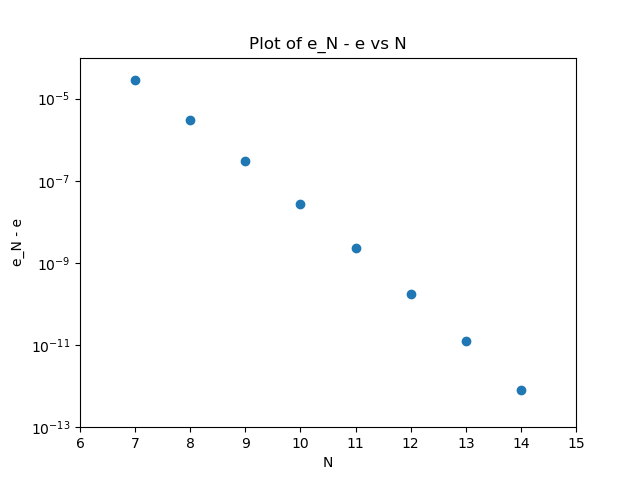
\includegraphics[scale=0.6]{e_n_vs_e.png}
        \caption{A plot of \(e_N - e\) against \(N\) showing how \(e_N\) becomes closer to \(e\) as \(N\) increases.}
    \end{figure}
    
    \subsection{Stability}
    Round off and truncation errors can amplify unwanted solutions to algorithms.
    For example consider the recursive function defined by
    \[f_n = f_{n - 1} + f_{n - 2}\]
    where \(f_0 = 1\) and \(f_1 = (1 - \sqrt{5})/2 \approx -0.618034\).
    What is the value, \(f_{\infty}\), of \(f_n\) as \(n\to\infty\)?
    To get an idea of what happens we compute a few values using the following code:\footnote{This code is actually very slow, it is better to store each value of \(f_n\) as it is calculated and use this whenever the value is needed, this makes computation significantly quicker.}
    \begin{lstlisting}[language=python]
    def f(n):
        if n == 0:
            return 1
        elif n == 1:
            return -0.618034
        return f(n - 1) + f(n - 2)
    \end{lstlisting}
    Doing this we get
    \[
        \begin{array}{c|c}
            n & f_n\\\hline
            5 & -0.09017\\
            10 & 0.008130\\
            15 & -0.0007400\\
            20 & \num{-1.000e-07}\\
            25 & \num{-8.500e-4}\\
            30 & \num{-9.361e-3}\\
            35 & -0.1038\\
            40 & -1.151\\
            45 & -12.77\\
            50 & -141.6\\
            55 & -1570\\
            60 & -17415\\
        \end{array}
    \]
    we see that the value hovers around 0 for a while and then drops off to negative infinity.
    The reason for this is that this recursion has a solution given by
    \[f_n = c_1\varphi^n + c_2(-\varphi)^{-n}.\]
    Where \(\varphi = (1 + \sqrt{5})/2 \approx 1.618034\) is the golden ratio.
    We chose initial values of \(f_0\) and \(f_1\) such that \(c_1 = 0\) and \(c_2 = 1\), however round off errors in the value of \(f_1\) caused \(c_1 < 0\) to be stored so once \(n\) becomes big enough the first term dominates and quickly tends towards \(-\infty\).
    
    A good numerical method should be stable, at least for some range of parameters.
    Errors should be suppressed instead of allowing them to compound and get bigger.
    
    \begin{figure}[ht]
        \centering
        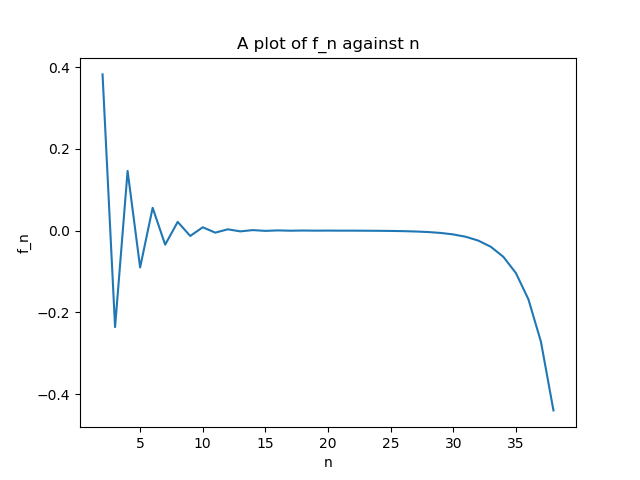
\includegraphics[scale=0.6]{fibonacci.png}
        \caption{A plot of \(f_n\) against \(n\), showing how \(f_n\) is stable at 0 for a while before falling to \(-\infty\).}
    \end{figure}
    
    \subsection{Complexity}
    Say an algorithm computes something for input data of size \(n\).
    The size could be the number of digits in a number or the length of the array or the number of pixels in an image.
    It is simply some useful measure of size for the problem at hand.
    We say that the complexity of the algorithm is \(O(f(n))\), where \(f\) is some function, if there exists a constant \(c\) such that the time taken to run the algorithm, \(T\), on an input of size \(n\) is bounded such that \(T < cf(n)\) for all \(n\).
    Common cases for \(f\) are \(n\), \(n^2\), \(\log n\), \(n\log n\), \(2^n\), and \(n!\).
    Only the fastest growing term of \(f\) is taken into account and any constant coefficients are dropped, so if \(f(n) = 5n^3 + 2n^2 + 7n + 8\) then the algorithm has complexity \(O(n^3)\).
    We can do this as we are interested in the behaviour of \(f\) as \(n \to \infty\).
    In this case this is completely determined by the \(n^3\) term.
    
    \begin{figure}[ht]
        \centering
        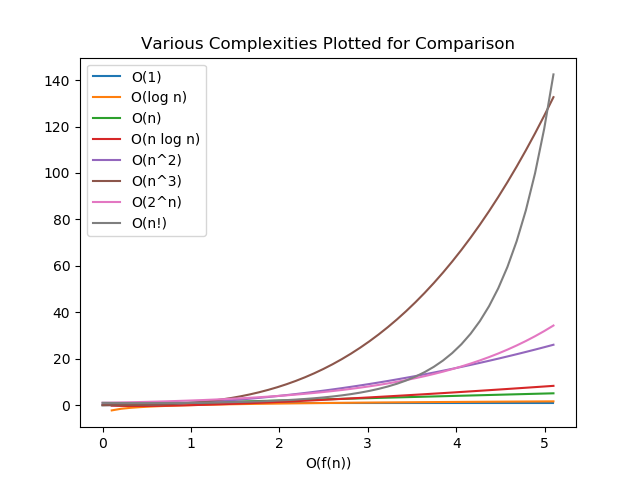
\includegraphics[scale=0.6]{complexities.png}
        \caption{Various complexities from \(O(1)\) to \(O(n!)\) plotted for comparison.}
    \end{figure}
    
    A single loop typically has \(O(n)\) complexity, for example the following is \(O(n)\):
    \begin{lstlisting}[language=python]
    total = 0
    for i in range(n):
        s += i
    \end{lstlisting}
    A double loop typically has \(O(n^2)\) complexity as for each item in the first loop the second loop must be completed \(n\) times and hence the second loop is computed \(n^2\) times.
    For example the following is \(O(n^2)\):
    \begin{lstlisting}[language=python]
    import numpy as np
    for i in range(n):
        for j in range(n):
            s += j * np.sin(0.1 * i)
    \end{lstlisting}
    The following is approximately three times faster, but still \(O(n^2)\), and it computes exactly the same thing:
    \begin{lstlisting}[language=python]
    import numpy as np
    for i in range(n):
        sin = np.sin(0.1 * i)
        for j in range(n):
            s += j * sin
    \end{lstlisting}
    It is much faster as \lstinline|np.sin(0.1 * i)| is only computed one time for each value of \(i\) rather than being computed one time for each value of \(j\).
    In general where possible put computation heavy steps outside as many of the loops as possible.
    This is still \(O(n^2)\) however as it is still a double loop.
    
    For some algorithms it is important to make a distinction between the typical/best-case/worst-case scenarios.
    For example quick sort is a common algorithm to sort an array of numbers.
    It has the following time complexities:
    \begin{itemize}
        \item Typical -- \(O(n\log n)\)
        \item Best-case -- \(O(n\log n)\)
        \item Worst-case -- \(O(n^2)\)
    \end{itemize}
    The worst case scenario actually occurs when the list is already sorted, or close to it.
    For this reason if you know that the list is likely to be almost in the correct order it may be better to use a different algorithm.
    
    \subsubsection{Why is Complexity Important?}
    Say we want to perform a \acrfull{dft} on a signal with \(n = \num{e9}\) samples.
    The first way we may think to do this, applying the formulas directly, ends up having a complexity of \(O(n^2)\).
    Thus if there are \(\num{e9}\) samples there are \((\num{e9})^2 = \num{e18}\) steps to this computation.
    If one step takes \(\SI{e-9}{\second}\) then the total time for execution of this algorithm is \(\SI{e9}{s} = \SI{32}{years}\).
    This is bad.
    
    Fortunately there exists an algorithm, called a \acrfull{fft}, that is \(O(n\log n)\).
    Then given \(\num{e9}\) samples there are about \(\num{e9}\ln\num{e9} \approx \num{2e10}\) steps.
    At \(\SI{e-9}{\second}\) per step the total execution time is \SI{20}{\second}.
    This is acceptable.
    
    \subsection{How to Achieve the Desired Degree of Accuracy}
    Numerical algorithms usually have some control parameter that determines the accuracy of the solution, \(x\).
    Sometimes this parameter directly specifies the allowable error, \(\delta x\).
    Usually it is more complicated.
    Going back to the example of \(e_N\) in section~\ref{sec:truncation errors} we have \(N\) as the control parameter.
    Say we want to find the value of \(e\) to ten decimal places.
    How can we do this given we don't know the true value of \(e\)?
    There is an almost universal approach to this problem:
    \begin{enumerate}
        \item Run the algorithm with some control parameter that we know to be too low, for our example we choose \(N = 5\).
        \item Increase the value and run the algorithm again, for our example we increase \(N\to N + 2\).
        \item Compare the last two results computed, if they differ by less than a certain amount stop.
        If not repeat the second step.
        For our example we want \(e_N - e_{N-1} < \num{e-10}\).
    \end{enumerate}
    Using this method we should find an acceptable value of \(N\).
    We actually overshoot slightly.
    A value of \(N = 13\) would be good enough but since we increase by 2 each time we stop at \(N = 14\).
    This isn't that big a deal as \(\sum_n1/n!\) is fairly fast to compute.
    Given a more time consuming algorithm we may choose to be more careful in the way we choose to increase \(N\).
    For example we may start with \(N \to 2N\) to find a rough value of \(N\) and then use \(N \to N + 1\) to find the most efficient value of \(N\).
    It is also better to run these tests with limited data sets where possible just for speed reasons.
    
    \begin{figure}[ht]
        \centering
        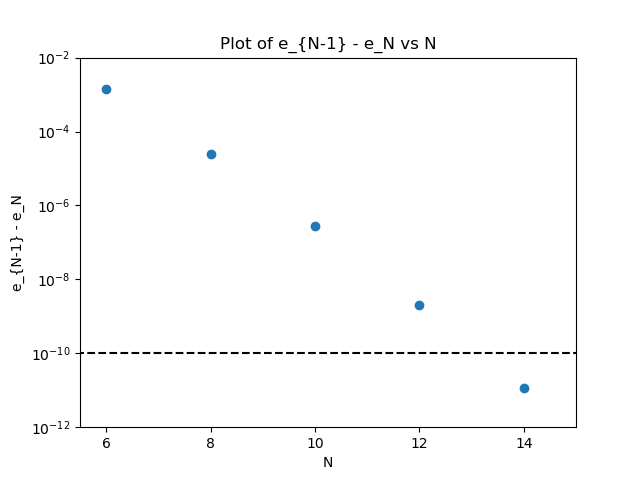
\includegraphics[scale=0.6]{e_n_vs_e_n-1.png}
        \caption{A plot of \(e_{N-1} - e_N\) vs \(N\), the difference is first seen to be below \(\num{e-10}\) at \(N = 14\).}
    \end{figure}

    \section{Ordinary Differential Equations}
    \Glspl{ode} are very common in physics and rarely have analytic solutions.
    Because of this solving an \gls{ode} is a very common numerical problem.
    The general problem is to solve the following equation:
    \begin{equation}\label{eqn:standard form ode}
        \dv{\vv{y}}{t} = f(\vv{y}, t),
    \end{equation}
    where \(\vv{y}\) and \(\vv{f}\) are \(n\)-dimensional vectors of functions, and we are also provided with some boundary conditions.
    It may seem like this only encompasses first order \glspl{ode} but it turns out that all \glspl{ode} can actually be written in this form.
    Consider, for example, a classic case of simple harmonic motion.
    This is described by
    \begin{equation}\label{eqn:shm}
        \dv[2]{x}{t} = -kx.
    \end{equation}
    By defining 
    \[v = \dv{x}{t}\]
    we can reduce equation~\ref{eqn:shm} to two first order \glspl{ode}:
    \[\dv{x}{t} = v,\qquad\text{and}\qquad \dv{v}{t} = -kx.\]
    Then by defining
    \[\vv{y} = (x, v), \qquad\text{and}\qquad \vv{f} = (y_2, -ky_1)\]
    we have reduced simple harmonic motion to solving an equation of the form of equation~\ref{eqn:standard form ode}.
    
    \subsection{Boundary Conditions}
    An \gls{ivp} is one of the two common ways in which boundary conditions are given.
    In an \gls{ivp} we know \(\vv{y}(t_0) = \vv{y_0}\) for some starting value \(t_0\).
    We want to know what \(\vv{y}(t)\) is for \(t > t_0\).
    
    A \gls{bvp} is the other common way in which boundary conditions are given.
    In a \gls{bvp} we know \(\vv{y}(t_0) = \vv{y_0}\) and \(\vv{y}(t_1) = \vv{y_1}\) with \(t_0 < t_1\).
    We want to find \(\vv{y}(t)\) for \(t \in [t_0, t_1]\).
    
    \subsection{Initial Value Problems}
    \subsubsection{Explicit Euler Method}
    The explicit Euler method (often just the Euler method) works by replacing derivatives with a finite definition, based on the definition of a derivative:
    \[\dv{y}{t} = \lim_{h\to 0} \frac{y(t + h) - y(t)}{h}.\]
    In the 1-dimensional case we approximate
    \[\dv{y}{t} = f(y, t)\]
    as
    \[\frac{y(t + h) - y(t)}{h} \approx f(y, t)\]
    where \(h\) is a small time step.
    Rearranging this we get
    \[y(t + h) \approx y(t) + hf(y, t).\]
    The algorithm for the explicit Euler method is then as follows:
    \begin{itemize}
        \item Set \(y_0\) to be the initial value.
        \item Calculate \(y_n = y(t + hn)\) recursively with
        \[y_{n+1} = y_n + hf(y_n, t).\]
    \end{itemize}
    This generalises easily to multiple dimensions, just replace \(y\) and \(f\) with \(\vv{y}\) and \(\vv{f}\).
    
    Essentially this algorithm comes down to assuming that the gradient of \(y\) between \(t\) and \(t + h\) is constant and therefore between these two points \(y\) can be given by a straight line and then uses this straight line to compute the value of \(y\) at \(t + h\).
    
    The error when using this method is typically of \(\order{h}\).
    
    An algorithm is stable if a small perturbation does not grow exponentially.
    For example if
    \[\dv{y}{t} = -cy\]
    with \(c < 0\) then the solution decays exponentially.
    The Euler method gives
    \[y_{n+1} = y_n - hcy_n = y_n(1 - hc).\]
    If \(\abs{1 - hc} < 1\) then a small perturbation will decrease exponentially as the prefactor \(y_n\) decreases exponentially.
    However if \(\abs{1 - hc} > 1\)  then a small perturbation increases exponentially and the algorithm is unstable.
    So in this case we have to pick \(h < 2/c\).
    The larger \(c\) is the smaller a value of \(h\) we have to pick to have a numerically stable algorithm.
    Obviously picking a smaller value of \(h\) means that we have to take more steps until we get to the point of interest and this means that the algorithm is much slower.
    
    Another example is the simple harmonic oscillator.
    We saw that this can be defined by the following pair of \glspl{ode}:
    \[\dv{y}{t} = v,\qquad\text{and}\qquad \dv{v}{t} = -y.\]
    If we apply the Euler method then we get that the amplitude of oscillation increases.
    This is non-physical as it violates conservation of energy.
    The Euler method in this case uses the following two recursion relations:
    \begin{align*}
        y_{n+1} &= y_n + hv_n,\\
        v_{n+1} &= v_{n+1} - hy_n.
    \end{align*}
    We can package these coupled equations nicely into one matrix equation:
    \[
        \begin{pmatrix}
            y_{n+1}\\ v_{n+1}
        \end{pmatrix}
        =
        \begin{pmatrix}
            1 & h\\
            -h & 1
        \end{pmatrix}
        \begin{pmatrix}
            y_n\\ v_n
        \end{pmatrix}
        .
    \]
    The matrix
    \[
        \begin{pmatrix}
            1 & h\\
            -h & 1
        \end{pmatrix}
    \]
    has two eigenvalues, \(\lambda_{\pm} = 1 \pm ih\).
    Iterating through the recursion relations to find \(y_n\) corresponds to raising this matrix to the power of \(n\).
    This amplifies terms in a way that is proportional to the largest absolute value of an eigenvalue.
    In this case both eigenvalues have the same absolute value so the solution will grow as \((\abs{\lambda_{\pm}})^n\).
    Since \(\abs{\lambda_{\pm}} > 1\) for all values of \(h\) this algorithm is never stable.
    
    In general the Euler method is rarely stable and when it is it often requires an impractically small value of \(h\).
    
    \subsubsection{Implicit Euler Method}
    The implicit Euler method is an improvement on the Euler method that uses a slightly different recursion relation:
    \[y_{n+1} = y_n + hf(y_{n+1}, t).\]
    Notice that the argument of \(f\) is now \(y_{n+1}\) instead of \(y_n\).
    Since \(y_{n+1}\) now appears on both sides of the equation, and \(f\) in general is non-linear, we need to use non-linear root finding to find \(y_{n+1}\) each iteration.
    We will cover non-linear root finding in the next section.
    
    Going back to the case of the harmonic oscillator again the matrix form of our recursion relation with the implicit Euler method is
    \[
        \begin{pmatrix}
            y_{n+1}\\ v_{n+1}
        \end{pmatrix}
        =
        \begin{pmatrix}
            y_n\\ v_n
        \end{pmatrix}
        +
        \begin{pmatrix}
            0 & h\\
            -h & 0
        \end{pmatrix}
        \begin{pmatrix}
            y_{n+1}\\ v_{n+1}
        \end{pmatrix}
        .
    \]
    Rearranging this gives us
    \[
        \begin{pmatrix}
            y_{n+1}\\ v_{n+1}
        \end{pmatrix}
        = \frac{1}{1 + h^2}
        \begin{pmatrix}
            1 & h\\
            -h & 1
        \end{pmatrix}
        \begin{pmatrix}
            y_n\\ v_n
        \end{pmatrix}
        .
    \]
    The eigenvalues of
    \[
        \frac{1}{1 + h^2}
        \begin{pmatrix}
            1 & h\\
            -h & 1
        \end{pmatrix}
    \]
    are
    \[\lambda_{\pm} = \frac{i}{i \pm h}.\]
    Now \(\abs{\lambda_{\pm}} < 1\) for all \(h\).
    This means that this algorithm is unconditionally stable.
    This doesn't mean we can use large values of \(h\) though, the error is still \(\order{h}\) its just that this error doesn't get worse as the algorithm progresses.
    
    In practice neither Euler method is used much as there are many other more accurate algorithms.
    Most of these are implicit in the same sense, that \(y_{n+1}\) appears on both sides of some recursion relation.
    
    \subsubsection{Second Order Runge--Kutta}
    The second order Runge--Kutta algorithm improves upon the Euler methods by taking a `trial step' to the midpoint of the interval.
    The algorithm is as follows:
    \begin{itemize}
        \item Set \(y = y_0\).
        \item Set
        \[k_1 = hf(y, t).\]
        \item Set
        \[k_2 = hf\left(y + \frac{k_1}{2}, t + \frac{h}{2}\right).\]
        \item Compute the recursion relation
        \[y(t + h) = y(t) + k_2.\]
    \end{itemize}
    This algorithm can be shown by taking the Taylor series and manipulating terms until we have the desired equation.
    We take up to terms in \(h^2\) for the Taylor series so the error on any one term is \(\order{h^3}\).
    This means that we can use larger values of \(h\) and get the same level of accuracy as the Euler methods.
    
    \subsubsection{Fourth Order Runge--Kutta}
    The fourth order Runge--Kutta algorithm (and indeed higher orders) is based on the same logic but taking more terms of the Taylor series.
    For the fourth order Runge--Kutta algorithm the algorithm is as follows:
    \begin{itemize}
        \item Set \(y = y_0\).
        \item Set
        \[k_1 = hf(y, t).\]
        \item Set
        \[k_2 = hf\left(y + \frac{k_1}{2}, t + \frac{h}{2}\right).\]
        \item Set
        \[k_3 = hf\left(y + \frac{k_3}{2}, t + \frac{h}{2}\right).\]
        \item Set
        \[k_4 = hf(y + k_3, t + h).\]
        \item Compute the recursion relation
        \[y(t + h) = y(t) + \frac{k_1}{6} + \frac{k_2}{3} + \frac{k_3}{3} + \frac{k_4}{6}.\]
    \end{itemize}
    The error on any one term is then \(\order{h^5}\).
    This method (and the fifth order Runge--Kutta) is very popular.
    It is especially good if the solution is smooth.
    This method is implemented in the \lstinline|scipy| module:
    \begin{lstlisting}[language=python]
    scpipy.integrate.solve_ivp(f, [t1, t2], y0, method="RK45")
    \end{lstlisting}
    In fact this is actually the default method for \lstinline[language=python]|solve_ivp|.
    If instead we want to use second order Runge--Kutta we can by setting \lstinline[language=python]|method="RK23"|.
    Note that \lstinline[language=python]|f| is expected to be a function of \lstinline[language=python]|t| and \lstinline[language=python]|y| in that order.
    
    
    \subsubsection{Explicit Euler vs. Fourth Order Runge--Kutta}
    In theory fourth order Runge--Kutta should be more accurate for the same value of \(h\).
    Fourth order Runge--Kutta has a global error of \(\order{h^4}\) and Euler has a global error of \(\order{h}\).
    Global error means the final error on the solution, as opposed to the error on one step along the way, which is typically smaller by a factor of \(h\).
    However the precise error depends on the problem at hand.
    For example solving
    \[\dv{y}{y} = y(1 - y), \qquad\text{where}\qquad y(0) = \frac{1}{2}\]
    the errors scale as we would expect for both algorithms.
    However when solving
    \[\dv{y}{t} = y\cos(t),\qquad\text{where}\qquad y(0) = 1\]
    the errors using Runge--Kutta and Euler both scale as \(\order{h}\).
    This is because of the explicit \(t\) dependence of \(f\).
    In general Runge--Kutta is less accurate when \(f\) depends explicitly on \(t\).
    
    \subsubsection{Adaptive Step Size Control}
    One way to improve on existing algorithms is with adaptive step size control.
    The general idea is to change the value of \(h\) as the algorithm progresses depending on the nature of \(f\) at the current point in the algorithm.
    One way to do this is with the following algorithm:
    \begin{itemize}
        \item Advance the solution from \(t\) to \(t + h\) with one of the above methods.
        \item Repeat with two steps of size \(h/2\), \(t \to t + h/2 \to t + h\).
        \item Compare the results, if the difference, \(\Delta y\), between the results is sufficiently small move on and increase \(h\) in the next step.
        If \(\Delta y\) is too large decrease \(h\) and try again.
    \end{itemize}
    The specifics of this algorithm differ in the routine used to advance the solution and how they change \(h\) in the last step.
    \lstinline[language=python]|solve_ivp| does this automatically.
    It may be necessary to set \lstinline[language=python]|max_step| which sets a maximum value for \(h\).
    This is because the value of \(h\) still affects the global accuracy.
    
    \subsubsection{Verlet Algorithm}
    In physics we often deal with equations of the form
    \[\dv[2]{\vv{x}}{t} = \vv{a}(\vv{x}(t))\]
    where a certain quantity (often energy) is conserved.
    The Euler and Runge--Kutta methods don't conserve this value.
    We saw this with the Euler method giving the non-physical solution to a harmonic oscillator of an ever increasing amplitude.
    
    The Verlet algorithm does preserve energy.
    One particular Verlet algorithm, called the velocity Verlet algorithm, is as follows:
    \[\vv{x}(t + h) = \vv{x}(t) + \vv{v}(t)h + \vv{a}(t)\frac{h^2}{2}\]
    \[\vv{v}(t + h) = \vv{v}(t) + \frac{1}{2}[\vv{a}(t + h) + \vv{a}(t)].\]
    Note that while this preserves the average energy it does oscillate slightly around this average value.
    This algorithm is not implemented in \lstinline[language=python]|scipy| so you would have to implement it yourself or use some other external library.
    
    \subsection{Boundary Value Problems}
    \subsubsection{Shooting Method}
    The goal of a \gls{bvp} is to solve an \gls{ode} of the form
    \[\dv{\vv{y}}{t} = \vv{f}(\vv{y}, t)\]
    where we know \(\vv{t}(t_1)\) and \(\vv{y}(t_2)\) for some \(t_2 > t_1\).
    The principle method by which we do this is to fix \(y_{n_1}, y_{n_2}, \dotsc\) at \(t_1\) and manipulate the rest of the initial values so that solving an \gls{ivp} with \(\vv{y}(t_1)\) as an initial value we also get the desired value of \(\vv{y}\) at \(t_2\), thus satisfying the boundary conditions.
    In general we will need non-linear root finding to apply this method.
    
    \begin{example}
        Say we want to solve the simple harmonic oscillator equations
        \[\dot{x} = v, \qquad\text{and}\qquad \dot{v} = -x, \qquad\text{where}\qquad, x(t_1) = x_1, \qquad\text{and}\qquad x(t_2) = x_2.\]
        To do this we solve \(x(t_2; v) = x_2\) for \(v\) where \(x(t_2; v)\) is the numerically obtained solution to the \gls{ivp} with the same equations and the condition \(x(t_1) = x_1\).
        To do this we simply try different values of \(v\) until one gives us a sufficiently close value to \(x_2\).
    \end{example}
    There is another popular method called the relaxation method but we will not discuss this yet as it requires \gls{pde} solving.
    The shooting method is implemented in the \lstinline[language=python]|scipy| module:
    \begin{lstlisting}[language=python]
    solve_bvp(f, bc, x_ini, y_ini)
    \end{lstlisting}
    
    \subsection{Potential Problems with \glspl{ode}}
    If we don't have enough boundary conditions then the solution will not be unique.
    Instead we will get a family of curves that satisfy the \gls{ode} and the boundary conditions we do have.
    
    Singularities can cause an issue, consider, for example, the \gls{ode}
    \[\dv{y}{t} = \frac{1}{1 - y}.\]
    This has a singularity at \(y = 1\).
    Trying any value greater than about \(t = 1/2\) will cause the solution to tend to this singularity.
    
    A stiff equation is one in which a certain term causes us to be forced to use a very small value of \(h\).
    For example
    \[\dv{u}{t} = 998y + 1998v,\qquad\text{and}\qquad \dv{v}{t} = -999u - 1999v.\]
    These equations have the explicit solutions
    \[u = 2e^{-t} - e^{-1000t},\quad\text{and}\qquad v = -e^{-t} + e^{-1000t}.\]
    The first terms here grow relatively slowly and the second grow relatively quickly.
    These second terms force \(h\) to be very small if we desire a stable algorithm, however they aren't actually that important for the behaviour of the function for large \(t\).
    However for stability we still need to take care of these components even if they don't actually affect the solution much.
    
    The final problem that one may have is chaos.
    Chaos is a property of a deterministic system in which a small change to initial conditions can greatly affect the outcome.
    There is no numerical method that can remove chaos but there are some that can amplify it's effect making it worse.
    The quintessential example of a chaotic system is the Lorentz system, which can be given by the following set of \glspl{ode}:
    \[x' = 10(-x + y),\qquad y' = 30x - y - xz,\qquad\text{and}\qquad z' = xy - 2z.\]
    
    \section{Root Finding}
    The general aim with root finding is to solve
    \[f(x) = 0.\]
    Where \(f\) is a non-linear function.
    In general \(x\) can be a single real number (1-dimensional root finding), a complex number (in which case we represent \(a + bi\) as a vector, \([a, b]\)), or a vector (multi-dimensional root finding).
    
    There are a few potential problems that we need to consider with every method:
    \begin{itemize}
        \item Multiple roots. 
        How do we find all of the roots/just the particular root that we care about?
        \item Discontinuities, for example \(f(x) = 1/x\), a lot of methods work by looking for a sign change in \(f(x)\) as \(x\) is slowly increased.
        Such a sign change occurs when moving from \(x < 0\) to \(x > 0\) for \(1/x\) but there is no root at \(x = 0\), instead there is a discontinuity.
        \item Near roots, for example \(f(x) = x^2 + 10^{-16}\) has no real roots but at \(x = 0\) it is very close to 0.
        Close enough that it is less than the precision of many floats.
    \end{itemize}
    
    \subsection{General Approach in One Dimension}
    Most methods start by choosing sensible initial values, either an approximate root, \(x\), or an interval, \([a, b]\), in which we think the root is.
    The better the initial guess is the quicker our method will converge.
    We then apply some iterative process to improve our guess repeatedly until our results are sufficiently close.
    
    \subsubsection{Bisection Method}\label{sec:bisection method}
    The most basic root finding method is the bisection method.
    However this is an important method as it is guaranteed to converge, although it may converge on a discontinuity.
    The general algorithm is as follows:
    \begin{itemize}
        \item Select an interval, \([a, b]\), in which the root is.
        Assuming that there is only one root in this interval we expect \(f(a)\) and \(f(b)\) to have opposite signs and so \(f(a)f(b) < 0\).
        \item Bisect the interval, find the midpoint:
        \[c = \frac{a + b}{2}.\]
        \item Check if the root is in the interval \([a, c]\) or \([c, a]\) by computing \(f(a)f(c)\) and \(f(c)f(b)\) respectively and seeing which is negative.
        Choose the interval that contains the root.
        \item Rename this interval to \([a, b]\) and repeat from the second step.
        Stop repeating once some condition has been satisfied, for example \(\abs{b - a} < \varepsilon\) where \(\varepsilon\) is some small value chosen as a maximum distance from the root at which the algorithm halts.
        Return the root:
        \[x_0 = \frac{a + b}{2}.\]
    \end{itemize}
    If there are no singularities in \([a, b]\), and, if there are multiple roots in \([a, b]\), we don't care which we find then this method will always succeed.
    Convergence is guaranteed in
    \[n = \log_2\frac{b - a}{\varepsilon}\]
    steps.
    Due to the slow rate of convergence we only use this method if all other methods fail.
    This method is not implemented in the \lstinline[language=python]|scipy| module:
    \begin{lstlisting}[language=python]
    scipy.optimize.bisect(f, a, b)
    \end{lstlisting}
    
    If the root cannot be bracketed by \([a, b]\) such that \(\sgn(f(a)) = -\sgn(f(b))\) then this method does not work.
    For example \(f(x) = x^2\) has a root at \(0\) but there is no way to bracket this as \(f(x) \ge 0\) for all \(x\).
    
    \subsubsection{Newton--Raphson}
    The approach of the Newton--Raphson method is to approximate a function near the root, \(x_0\), by its Taylor series:
    \[f(x_0) \approx f(x) + (x_0 - x)f'(x).\]
    We then set \(f(x_0) = 0\) as \(x_0\) is a root an rearrange to get
    \[x_0 \approx x - \frac{f(x)}{f'(x)}.\]
    The general algorithm for using this to find the root is then
    \begin{itemize}
        \item Guess the value of \(x_0\).
        \item Recursively calculate
        \[x_n = x_{n-1} - \frac{f(x_{n-1})}{f'(x_{n-1})}.\]
        \item Repeat until \(\abs{x_{n} = x_{n-1}} < \varepsilon\).
    \end{itemize}
    This method is implemented in the \lstinline[language=python]|scipy| module:
    \begin{lstlisting}[language=python]
    scipy.optimize.newton(func, x0, fprime)
    \end{lstlisting}
    This method doesn't always converge so it is not recommended.
    It also needs the derivative which we don't necessarily know and may be computationally expensive to compute.
    
    \subsubsection{Secant Method}
    The secant method is a way around not having the derivative with the Newton--Raphson method.
    It works by replacing the derivative with a finite difference.
    The algorithm is as follows:
    \begin{itemize}
        \item Guess an interval, \([x_1, x_2]\), which contains the root, \(x_0\).
        \item Recursively compute
        \[x_n = x_{n-1} - f(x_{n-1})\frac{(x_{n-1} - x_{n-2})}{f(x_{n-1}) - f(x_{n-2})}.\]
        \item Repeat until \(\abs{x_n - x_{n-1}}<\varepsilon\).
    \end{itemize}
    This method has all the issues of the Newton--Raphson method as well as extra error caused by approximating the derivative.
    It is implemented in \lstinline[language=python]|scipy| by using
    \begin{lstlisting}[language=python]
    scipy.optimize.newton(func, x0, x1=x1)
    \end{lstlisting}
    That is the same as the Newton--Raphson method but instead of giving it the derivative we give it a second value of \(x\).
    
    \subsubsection{Brent's Method}
    The Newton--Raphson and secant methods are not guaranteed to converge but when they do are much faster than bisection.
    Brent's method combines the two, bisection is used far from the root and nearer the root the secant method or similar is used.
    This is guaranteed to converge and is faster than bisection alone.
    
    This is implemented in \lstinline[language=python]|scipy| as
    \begin{lstlisting}[language=python]
    scipy.optimize.brentq(f, a, b)
    \end{lstlisting}
    Here the \lstinline[language=python]|q| stands for quadratic interpolation which is the method used when near the root.
    This should be the method of choice for most 1-dimensional, non-linear, root finding problems.
    
    \subsection{Multi-Dimensional Root Finding}
    If we want to solve
    \[f(\vv{x}) = 0,\]
    where \(\vv{x}\) is a vector of \(N\) variables, then things become significantly harder.
    For one we no longer necessarily have single solutions.
    Consider \(x_1^2 + x_2^2 - 1 = 0\).
    This has as a solution the unit circle, \(S^1\).
    This means that there are an infinite number of roots.
    In general the roots to a single equation form a hyperplane of dimension \(N-1\).
    The question is which of these roots the algorithm will find.
    
    In the most general case we can allow \(\vv{f}\) to be a vector of functions.
    For example
    \begin{equation}
        f_1(\vv{x}) = \frac{1}{2}x_1^2 + 2x_2^2 - 1 = 0\\
        f_2(\vv{x}) = \frac{1}{2}x_1^2 + \frac{1}{2}x_2^2 - 1 = 0.
    \end{equation}
    These equations describe a pair of ellipses that overlap a finite number of times (four times to be precise).
    This actually solves the problem of an infinite number of roots but in general as the dimension increases the problem of an infinite number of roots only gets worse.
    Problems with a large number of dimensions are very common in physics.
    For example if we want to model a large \((\sim\num{e6})\) number of particles in some non-linear potential then each particle needs 3 equations of motion in 3-dimensions resulting in \(N = \num{3e6}\).
    
    \subsubsection{Multi-Dimensional Newton--Raphson}
    This method starts with the Taylor expansion of \(\vv{f}\):
    \[\vv{f}(\vv{x} + \delta\vv{x}) \approx \vv{f}(\vv{x}) + J\delta\vv{x}\]
    where \(J\) is the Jacobian matrix:
    \[J_{ij} = \dv{f_i}{x_j}.\]
    
    If there is a root at approximately \(\vv{x} + \delta\vv{x}\) then
    \[0 \approx \vv{f}(\vv{x}) + J\delta\vv{x}.\]
    The algorithm for finding the root is then as follows:
    \begin{itemize}
        \item Guess \(\vv{x}\).
        \item Find \(\delta\vv{x}\) by solving the linear system
        \[J\delta\vv{x} = -\vv{f}(\vv{x}) \implies \delta\vv{x} = J^{-1}\vv{f}(\vv{x}).\]
        \item Set \(\vv{x} = \vv{x} + \delta\vv{x}\).
        \item Repeat until \(\abs{\delta\vv{x}} < \varepsilon\).
    \end{itemize}
    Compare this with the 1-dimensional Newton--Raphson method, there the Jacobian is simply the derivative, \(J = f'(x)\), and \(\delta x\) is \(-J^{-1}f(x) = f(x)/f'(x)\).
    We will look at how to find inverse matrices for large matrices in a later section.
    
    Often computing \(J\) is impossible/inconvenient.
    In this case we can use Broyden's method.
    This method is allows us to compute the Jacobian once rather than at every step, so even if it is computationally expensive it is still possible.
    The algorithm is as follows:
    \begin{itemize}
        \item Guess \(\vv{x}_1\) and \(J_1\).
        \item Recursively calculate
        \[J_n = \frac{J_{n-1} + \delta f_n - J_{n-1} - J_{n-1}\delta\vv{x}_n}{\abs{\delta\vv{x}_n}^2}\delta\vv{x}\trans,\]
        and
        \[\vv{x}_{n+1} = \vv{x}_n - J_{n}^{-1}\vv{f}(\vv{x}_n),\]
        where
        \[\delta\vv{f}_n = \vv{f}(\vv{x}_n) - \vv{f}(\vv{x}_{n-1})\]
        and
        \[\delta\vv{x}_n = \vv{x}_n - \vv{x}_{n-1}.\]
    \end{itemize}
    This is implemented in the \lstinline[language=python]|scipy| module:
    \begin{lstlisting}[language=python]
    scipy.optimize.root(fun, x0, method=broyden1)
    \end{lstlisting}
    There is another modification to this method that means that we don't need to compute \(J^{-1}\) but we won't discuss it here.
    
    Sometimes this method converges to a value that solves only one, or some, of the equations, \(f_i\) but not all.
    Sometimes it converges to non-solutions.
    The root to which the algorithm converges is non-trivially related to the initial value chosen.
    This means that the method doesn't necessarily converge to the closest root.
    
    \subsection{Selecting The Best Algorithm}
    In one dimension Brent's method is usually the best choice.
    There may be special cases where the derivative can be calculated and the root guessed to high accuracy where Newton--Raphson is the best method.
    If all else fails bisection should work.
    
    In \(N\) dimensions if the root is known approximately then Newton-Raphson should be used if the Jacobian is known or Broyden's method if it isn't.
    
    In \(N\) dimensions if the root is not known then a hybrid method that combines minimisation (which we will cover later in the course) to find the approximate root and then a root finding algorithm is the best method to use.
    
    \subsection{Numerical Calculations and Hardware}
    The \gls{cpu} is where most computation is done on a computer.
    It is physically separated from the hard drive where the memory is.
    For this reason it takes time to fetch data from the memory.
    To get around this problem most computers have a cache that is near the \gls{cpu}.
    This cache can store a small amount of data for fast access.
    However the size of the cache is not always that large.
    A well written program can exploit this and a badly written one can be much slower for not taking advantage of it.
    Consider the two following programs which have the same outputs.
    In both \lstinline[language=python]|a| is an \(n\times n\) array.
    \begin{multicols}{2}
    \begin{lstlisting}[language=python]
    for i in range(n):
        for j in range(n):
            a[i][j] += 1
    \end{lstlisting}
    \begin{lstlisting}[language=python]
    for i in range(n):
        for j in range(n):
            a[j][i] += 1
    \end{lstlisting}
    \end{multicols}
    The only difference is that the first has \lstinline[language=python]|x[i][j]| and the second has \lstinline[language=python]|x[j][i]|.
    However for large \(n\) the first is considerably faster.
    This is because of how arrays are stored in memory.
    Arrays are stored in continuous memory blocks so that the addresses of elements that are close in the array are close in memory space.
    When we access \lstinline[language=python]|x[0][0]| the array nearby is moved into the cache.
    If the next access is \lstinline[language=python]|x[0][1]| then this is already in the cache.
    However if the next access is \lstinline[language=python]|x[1][0]| and the array is large enough that a whole row doesn't fit in the cache at once then this is not yet cached so the whole caching process has to start again.
    
    \section{Interpolation and Integration}
    \subsection{Interpolation}
    Suppose we have a set of data points, \(\{(x_i, y_i)\st i = 1, \dotsc, N\}\).
    If we need points in between these, say at some point \(x\notin\{x_i\st i = 1, \dotsc, N\}\), and for some reason cannot compute \(y = y(x)\) then the process we use to estimate \(y\) is called interpolation.
    To do this we assume that the data can be represented by a smooth function between data points.
    We look for a function that goes through all of the points and that we can evaluate between points.
    
    This is not the same as curve fitting.
    When we fit a curve to some data we assume that the points approximate a nice smooth function with some error.
    The curve does not go through all points, it simply minimises some method of measuring distance from the points, such as least squares.
    Information is lost when we fit a curve but not when we interpolate.
    
    Interpolation also shouldn't be used to extrapolate beyond the edges of the data we have.
    There is no guarantee that the interpolated curve will make sense outside of the given data range.
    
    \subsection{Linear Interpolation}
    The simplest interpolation assumes that the data points, \(\{(x_i, y_i)\}\), are connected by a straight line.
    We also assume that we have a sorted array \([x_1, \dotsc, x_N]\)  such that \(x_i < x_{i+1}\) for all \(i\).
    The gradient between \(x_i\) and \(x_{i+1}\) is then
    \[m = \frac{y_{i+1} - y_i}{x_{i+1} - x_i}.\]
    The equation for a straight line is
    \[y - y_i = m(x - x_i),\]
    which gives us
    \[y(x) = y_i + \frac{(x - x_i)}{x_{i+1} - x_i}(y_{i+1} - y_i).\]
    We also need to find the correct value of \(i\) for a given \(x\).
    To do this we assume that \([x_1, \dotsc, x_n]\) is sorted and perform a binary search:
    \begin{lstlisting}[language=python]
    x_values = [x_1, ..., x_n]
    i_bottom = 1
    i_top = N
    while i_top - i_bottom > 1:
        i = int((i_top + i_bottom) / 2)
        if x_values[i] > x:
            i_top = i
        else:
            i_bottom = i
    i = i_bottom
    \end{lstlisting}
    This method is \(\order{\ln n}\) to find the correct value of \(i\), and \(\order{1}\) to compute \(y(x)\) once we have the correct value of \(i\).
    If \([x_1, \dotsc, x_n]\) is not sorted then it will need to be sorted.
    The inbuilt sort method for an array is \(\order{n\log n}\).
    A linear interpolation method is implemented in \lstinline|scipy|:
    \begin{lstlisting}
        scipy.interpolate.interp1d(x, y)
    \end{lstlisting}
    This function expects \lstinline|x| and \lstinline|y| to be arrays of paired \(x\) and \(y\) values.
    It returns a function that can be used to compute any value of \(y(x)\) for \(x\in[x_1, x_N]\).
    
    One problem with linear interpolation is that unless the data lie on a straight line the derivative of the piecewise function does not exist at the points \(x_i\).
    
    \subsection{Lagrange's Interpolating Polynomial}
    To have derivatives exist everywhere we use higher order polynomials.
    One way is to use a polynomial of order \(N - 1\) called Lagrange's interpolating polynomial, it is given by
    \begin{align*}
        y(x) &= \frac{(x - x_2)(x - x_3)\dotsm(x - x_N)}{(x_1 - x_2)(x_1 - x_3)\dotsm(x_1 - x_N)}y_1 + \frac{(x - x_1)(x - x_2)\dotsm(x - x_N)}{(x_2 - x_1)(x_2 - x_3)\dotsm(x_2 - x_N)}y_2 + \dotsb \\&\qquad+ \frac{(x - x_1)(x - x_2)\dotsm(x - x_{N-1})}{(x_N - x_1)(x_N - x_2)\dotsm(x_N - x_{N-1})}y_N\\
        &= \sum_{i=1} y_i \prod_{\stackrel{j=1}{j\ne i}}^{N} \frac{(x - x_j)}{x_i - x_j}
    \end{align*}
    This method is not good for large \(N\), it is \(\order{N^2}\).
    In the case that \(N = 2\) this method reduces to linear interpolation.
    This method is particularly bad for extrapolation.
    
    \subsection{Cubic Splines}
    A good middle ground is to use a third order polynomial.
    The most common way to do this is with a method called cubic splines.
    For \(x\in(x_i, x_{i+1})\) we compute \(y(x)\) as
    \[y(x) = s_i(x) = a_i + b_it + c_it^2 + d_it^3\]
    where
    \[t = \frac{x - x_i}{x_{i+1} - x_i}.\]
    We demand that the following equalities hold:
    \begin{align*}
        s_i(x_i) &= y_i,\\
        s_i(x_{i+1}) &= y_{i+1},\\
        s_i'(x_i) &= s_{i-1}(x_i),\\
        s_i'(x_{i+1}) &= s_{i+1}'(x_i),\\
        s_i''(x_{i+1}) &= s_{i+1}''(x_i),\\
        s_1''(x_1) &= 0,\\
        s_N''(x_N) &= 0.
    \end{align*}
    This gives a set of linear tridiagonal equations in \(\{a_i, b_i, c_i, d_i\}\).
    What this means is that written as a matrix the leading diagonal and the diagonals directly above and below it contain the only non-zero entries.
    For example the following is a tridiagonal matrix:
    \[
        \begin{bmatrix}
            \alpha & \beta & 0 & 0 & 0 & 0\\
            \gamma & \delta & \varepsilon & 0 & 0 & 0\\
            0 & \zeta & \eta & \vartheta & 0 & 0\\
            0 & 0 & \iota & \kappa & \lambda & 0\\
            0 & 0 & 0 & \mu & \nu & \xi\\
            0 & 0 & 0 & 0 & o & \pi\\
        \end{bmatrix}
        =
        \begin{bmatrix}
            \alpha & \beta &  &  &  & \\
            \gamma & \delta & \varepsilon &  & 0 & \\
             & \zeta & \eta & \vartheta &  & \\
             &  & \iota & \kappa & \lambda & \\
             & 0 &  & \mu & \nu & \xi\\
             &  &  &  & o & \pi\\
        \end{bmatrix}
        .
    \]
    This method is \(\order{N}\) to calculate the coefficients, \(\order{\log N}\) to find the correct value of \(i\) and \(\order{1}\) to compute \(s_i(x)\).
    This is a very popular method and generalises to more dimensions.
    It is implemented in \lstinline|scipy| as
    \begin{lstlisting}
    scipy.interpolate.interp1d(x, y, kind="cubic")
    \end{lstlisting}

    \subsection{When to Interpolate}
    Interpolate if:
    \begin{itemize}
        \item Data comes from a smooth function,
        \item The function is expensive to calculate (either computationally or the data comes from an experiment).
    \end{itemize}
    When interpolating:
    \begin{itemize}
        \item Use cubic splines,
        \item Unless speed/simplicity is important, then use linear interpolation,
        \item Don't use higher order polynomials.
    \end{itemize}
    Don't interpolate if:
    \begin{itemize}
        \item The data is noisy, smoothen the data first or fit a curve with fewer parameters,
        \item The data is in a lot of dimensions, there will be too many possible functions between data points.
    \end{itemize}
    
    \subsection{Integration}
    Only definite integrals give a numerical answer so this is the only sort that we will be looking at.
    The general problem is to find
    \[I = \int_a^b f(x)\dd{x}.\]
    The general strategy is
    \begin{itemize}
        \item Divide \([a, b]\) into a large number, \(N\), of smaller intervals, \([x_0, x_1], [x_1, x_2], \dotsc, [x_{N-1}, x_N]\) where \(x_0 = a\) and \(x_N = b\).
        \item Evaluate \(f(x)\) at points \(x_i\).
        \item Interpolate \(f(x)\) in each subinterval with a simple polynomial that can be integrated exactly.
        \item Add up contributions from the exact integrals over each \([x_i, x_{i+1}]\).
    \end{itemize}
    The precise interpolation method is where most algorithms vary.
    
    \subsubsection{Trapezoid Rule}
    The trapezoid rule uses linear interpolation.
    It also assumes that the \(x_i\) are a constant distance, \(h\), apart.
    This results in the area in \([x_i, x_{i+1}]\) under this linear interpolation is a trapezoid.
    The total area under all trapezoids is then
    \[I \approx h\left(\frac{1}{2}f_0 + f_1 + \dotsb + f_{N-1} + \frac{1}{2}f_N\right)\]
    where
    \[f_i = f(a + ih),\qquad\text{and}\qquad h = \frac{b - a}{N}.\]
    The error, defined as the absolute value of the difference between the actual integral and the estimated integral, drops off as \(1/N^2\).
    
    This is implemented in \lstinline|scipy|:
    \begin{lstlisting}
    scipy.integrate.trapz(y, x=None, dx=h)
    \end{lstlisting}
    This function expects \(y\) to be an array of values of \(f_i\).
    
    \subsubsection{Simpson's Rule and Cubic Interpolation}
    Simpson's rule is similar to the trapezoid rule but
    \[I \approx h\left(\frac{1}{3}f_1 + \frac{4}{3}f_2 + \frac{4}{3}f_3 + \dotsb + \frac{4}{3}f_{N-1} + \frac{1}{3}f_N\right).\]
    For optimal performance \(N\) should be even.
    
    Cubic interpolation is, again, similar but
    \[I \approx h\left(\frac{3}{8}f_0 + \frac{7}{6}f_1 + \frac{23}{24}f_2 + f_3 + f_4 + \dotsb + f_{N-4} + f_{N-3} + \frac{23}{24}f_{N-2} + \frac{7}{6}f_{N-2} + \frac{3}{8}f_N\right).\]
    
    For both Simpson's rule and cubic interpolation the error drops off as \(1/N^4\).
    These also assume a fairly smooth function, \(f\).
    If this isn't the case then trapezoid rule can be better as the error is also proportional to some higher order derivatives.
    
    Simpson's rule is implemented in \lstinline|scipy|:
    \begin{lstlisting}
    scipy.integrate.simps(y, x=None, dx=h)
    \end{lstlisting}
    
    \subsubsection{Adaptive Integration}
    The general idea behind adaptive integration is that in areas where the function, \(f\), changes slowly it is unnecessary to use lots of intervals whereas if \(f\) changes quickly we need more intervals.
    This can be implemented as a recursive function:
    \begin{lstlisting}
    def adaptive_int(f, a, b, max_ error):
        I, error = integrate(f, a, b)
        if error > max_error:
            m = (a + b) / 2
            I = addaptive_int(f, a, m, max_error / 2) + \
                addaptive_int(f, m, b, max_error / 2)
        return I
    \end{lstlisting}
    This function assumes the existence of some method, \lstinline|integrate| which could use the trapezoid rule or some other integration routine to calculate the integral of \lstinline|f| between \lstinline|a| and \lstinline|b|.
    \lstinline|max_error| is some maximum amount of error that we will accept.
    
    One problem with this method is it may miss sharp features by having intervals be too long.
    If you know that your function will have sharp features it is best to split the integral at each sharp feature and then integrate between these points and add the resulting integrals together.
    
    \subsubsection{Improper Integrals}
    There are two types of improper integrals.
    For the first  \(a, b = \pm\infty\) and for the second \(f\) has integrable singularities in \([a, b]\).
    In both cases the problem may be able to be fixed by a substitution that removes infinities.
    If \(a, b = \pm\infty\) then if \(f\) decays sufficiently quickly, for example \(f(x) = e^{-x}\), then it may be possible to approximate infinity with some large value:
    \[\int_0^\infty e^{-x}\dd{x} = 1, \qquad\text{and}\qquad \int_0^{100} e^{-x}\dd{x} = 0.99999999999999999999999999999999999999999996.\]
    The function \lstinline|scipy.integrate.quad(f, a, b)| accepts \lstinline|a| and \lstinline|b| as \(\pm\)\lstinline|np.inf|.
    
    \subsubsection{Oscillatory Integrals}
    An oscillatory integral, such as an integral of \(\sin(\omega x)f(x)\), can be computed with the methods discussed here but there are also specialised methods that exist and are often better, in particular  if \(f\) changes very slowly compared to the oscillatory term.
    These integrals are common with harmonic oscillators and Fourier transforms.
    
    \subsubsection{Multi-Dimensional Integrals}
    In general a \(d\)-dimensional integral, for relatively small values of \(d\), can be computed by recursively computing 1-dimensional integrals.
    For example
    \[I = \int_a^b \int_c^d f(x, y)\dd{x}\dd{y}\]
    can be computed by computing
    \[\int_a^b g(y)\dd{y}\]
    with
    \[g(y) = \int_c^d f(x, y)\dd{x}.\]
    Importantly if we need \(N\) points to achieve the desired degree of accuracy in one dimension then in \(d\) dimensions we need \(N^d\) points.
    
    If \(d\) is large then it is better to use Monte Carlo methods which we will cover in a later section.
    
    The following methods are implemented in \lstinline|scipy|:
    \begin{lstlisting}
    scipy.integrate.dblquad(f, a, b, g, h)
    scipy.integrate.tplquad(f, a, b, g, h, q, r)
    scipy.integrate.nquad(f, ranges)
    \end{lstlisting}
    The first implements a double integral of the form
    \[I = \int_a^b \int_{g(x)}^{h(x)}f(x, y)\dd{y}\dd{x}\]
    and the second implements a triple integral of the form
    \[I = \int_a^b \int_{g(x)}^{h(x)}\int_{q(x, y)}^{r(x, y)} f(x, y, z) \dd{z}\dd{y}\dd{x}.\]
    The third is similar.
    
    \subsubsection{Selecting an Integration Method}
    \begin{itemize}
        \item Smooth function -- use adaptive integration
        \item Sharp features -- determine their positions and split the integral at these points
        \item Oscillatory integral -- use a special method
        \item Special functions, such as Euler's gamma function, Gaussians, etc. -- use special methods
        \item Multi-dimensional:
        \begin{itemize}
            \item Reduce to one dimension if possible
            \item If not then use a
            \begin{itemize}
                \item recursive approach, \(d = 2, 3\)
                \item Monte Carlo method, \(d > 3\)
            \end{itemize}
        \end{itemize}
    \end{itemize}
    The \lstinline|scipy.integrate.quad| method attempts to choose the best method from a certain range of implemented methods.
    
    \section{Linear Algebra}
    \subsection{Common Problems}
    There are two common problems in linear algebra that we solve numerically.
    The first is solving a system of \(N\) linear equations with \(N\) unknowns for some large \(N\).
    This is common as a subroutine for other numerical methods such as spline interpolation, solving differential equations, or optimisation.
    
    The other problem we often have is diagonalising an \(N\times N\) matrix, that is finding it's eigenvalues and eigenvectors.
    This is common in quantum mechanics/quantum field theory as observables are directly related to the eigenvalues of operators.
    It also occurs often in statistical mechanics when solving master equations for many particles.
    This is also important in data analysis and many other fields.
    
    Most routines discussed in this section are implemented in \lstinline|scipy.linalg|.
    
    \subsection{Types of Matrices}
    Many routines are optimised for certain types of matrices.
    One way of classifying matrices is by the proportion of non-zero elements:
    \begin{itemize}
        \item Dense matrices -- Any matrix with a finite fraction of non-zero elements (finite in the sense that as \(N\to\infty\) for matrices of this form the fraction of non-zero entries does not go to zero).
        \begin{itemize}
            \item Upper/lower triangle matrices -- These matrices are non-zero only above/below and on the leading diagonal.
            For example \(U\) and \(L\) are upper and lower matrices respectively:
            \[
                U = 
                \begin{bmatrix}
                	U_{11} & U_{12} & U_{13} & U_{14} \\
                	0      & U_{22} & U_{23} & U_{24} \\
                	0      & 0      & U_{33} & U_{34} \\
                	0      & 0      & 0      & U_{44}
                \end{bmatrix}
                =
                \begin{bmatrix}
                    U_{11} & U_{12} & U_{13} & U_{14} \\
                           & U_{22} & U_{23} & U_{24} \\
                           &        & U_{33} & U_{34} \\
                    0      &        &        & U_{44}
                \end{bmatrix}
                ,
            \]
            and
            \[
                L = 
                \begin{bmatrix}
                	L_{11} & 0      & 0      & 0      \\
                	L_{21} & L_{22} & 0      & 0      \\
                	L_{31} & L_{32} & L_{33} & 0      \\
                	L_{41} & L_{42} & L_{43} & L_{44}
                \end{bmatrix}
                =
                \begin{bmatrix}
                    L_{11} &        &        & 0      \\
                    L_{21} & L_{22} &        &        \\
                    L_{31} & L_{32} & L_{33} &        \\
                    L_{41} & L_{42} & L_{43} & L_{44}
                \end{bmatrix}
                .
            \]
            
            \item Vandermonde matrix -- Each row has the elements of a geometric progression starting at one:
            \[
                V =
                \begin{bmatrix}
                	1 & a & a^1 & a^3 \\
                	1 & b & b^2 & b^3 \\
                	1 & c & c^2 & c^3 \\
                	1 & d & d^2 & d^3
                \end{bmatrix}
                .
            \]
            
            \item Toeplitz matrix -- Each diagonal is a constant:
            \[
                T =
                \begin{bmatrix}
                	a & b & c & d \\
                	e & a & b & c \\
                	f & e & a & b \\
                	g & f & e & a
                \end{bmatrix}
                .
            \]
        \end{itemize}
        
        \item Sparse matrices -- Any form of matrix where, as \(N\to\infty\), the fraction of non-zero elements goes to zero.
        
        \begin{itemize}
            \item Diagonal matrix -- Only the leading diagonal has non-zero elements:
            \[
                D =
                \begin{bmatrix}
                	D_{11} & 0      & 0      & 0      \\
                	0      & D_{22} & 0      & 0      \\
                	0      & 0      & D_{33} & 0      \\
                	0      & 0      & 0      & D_{44}
                \end{bmatrix}
                =
                \begin{bmatrix}
                    D_{11} &        &        & 0      \\
                           & D_{22} &        &        \\
                           &        & D_{33} &        \\
                    0      &        &        & D_{44}
                \end{bmatrix}
                .
            \]
            These are sparse as they have at most \(N\) non-zero elements so in the limit as \(N \to \infty\) the fraction of non-zero elements is
            \[\lim_{N\to\infty} \frac{N}{N^2} = \lim_{N\to\infty}\frac{1}{N} = 0.\]
            
            \item Tridiagonal matrices -- Only the leading diagonal and the diagonals directly above and below it have non-zero elements:
            \[
                T =
                \begin{bmatrix}
                	T_{11} & T_{12} & 0      & 0      \\
                	T_{21} & T_{22} & T_{23} & 0      \\
                	0      & T_{32} & T_{33} & T_{34} \\
                	0      & 0      & T_{43} & T_{44}
                \end{bmatrix}
                .
            \]
            These are sparse as they have at most \(3N - 2\) non-zero elements (notice that the first and last row have only 2 non-zero elements and the rest have 3).
            Thus as \(N\to\infty\) the fraction of non-zero elements is
            \[\lim_{N\to\infty}\frac{3N - 2}{N^2} = \lim_{N\to\infty}\left(\frac{3}{N} - \frac{2}{N^2}\right) = 0.\]
            
            \item Band diagonal matrices -- The logical generalisation from diagonal to tridiagonal and again to band matrices.
            The non-zero elements are only on the leading diagonal and some small (relative to \(N\)) number of diagonals above and below.
            
            \item Block diagonal matrix -- Combines two types of matrices a block matrix can be broken up into sub-matrices and for a block diagonal matrix this can be done in such a way that the resulting matrix of sub-matrices is diagonal:
            \[
                B = 
                \begin{bmatrix}
                	W_{11} & 0      & 0      & 0      & 0      & 0      \\
                	0      & X_{11} & X_{12} & 0      & 0      & 0      \\
                	0      & X_{21} & X_{22} & 0      & 0      & 0      \\
                	0      & 0      & 0      & Y_{11} & Y_{12} & 0      \\
                	0      & 0      & 0      & Y_{21} & Y_{22} & 0      \\
                	0      & 0      & 0      & 0      & 0      & Z_{11}
                \end{bmatrix}
                =
                \begin{bmatrix}
                	W & 0 & 0 & 0 \\
                	0 & X & 0 & 0 \\
                	0 & 0 & Y & 0 \\
                	0 & 0 & 0 & Z
                \end{bmatrix}
                .
            \]
        \end{itemize}
    \end{itemize}
    Another common way to categorise matrices is by their algebraic properties.
    Most of these relate to the transpose, defined as
    \[[A\trans]_{ij} = A_{ji},\]
    and Hermitian conjugate, defined as
    \[[A\hermit]_{ij} = A_{ji}^* = {A\trans}^*.\]
    \begin{itemize}
        \item Symmetric and Hermitian matrices:
        \[S\trans = S,\qquad\text{and}\qquad H\hermit = H.\]
        \item Orthogonal and unitary matrices:
        \[O\trans O = OO\trans = \ident,\qquad\text{and}\qquad U\hermit U = UU\hermit = \ident.\]
        \item Normal matrices:
        \[N\hermit N = NN\hermit.\]
    \end{itemize}

    \subsection{Linear Equations With Triangular Matrices}
    Suppose we have a set of linear equations that can be encoded in the form
    \[A\vv{x} = \bb{b}\]
    where \(A\) is an upper triangular matrix and \(\vv{b}\) is an \(N\)-dimensional vector of known values and \(\vv{x}\) is an \(N\)-dimensional vector of unknowns:
    \[
        \begin{bmatrix}
        	A_{11} & A_{12} & A_{13} & \dots  & A_{1N}    \\
        	0      & A_{22} & A_{23} & \dots  & A_{2N}    \\
        	0      & 0      & A_{33} & \dots  & A_{3N}    \\
        	\vdots & \vdots & \vdots & \ddots & \vdots    \\
        	0      & 0      & 0      & \dots  & A_{N-1,N} \\
        	0      & 0      & 0      & \dots  & A_{NN}
        \end{bmatrix}
        \begin{bmatrix}
            x_1\\ x_2\\ x_3\\ \vdots\\ x_{N-1}\\ x_N
        \end{bmatrix}
        =
        \begin{bmatrix}
            b_1\\ b_2\\ b_3\\ \vdots\\ b_{N-1}\\ b_N
        \end{bmatrix}
        .
    \]
    Equations that can be written like this are relatively easy to solve.
    By inspection we can see that we must have
    \[A_{NN}x_N = b_N \implies x_N = \frac{b_N}{A_{NN}}.\]
    We can then use back substitution to compute \(x_{N-1}\) by noting that
    \[A_{N-1,N-1} x_{N-1} + A_{N-1,N}x_N = b_{N-1} \implies x_{N-1} = \frac{b_{N-1} - A_{N-1,N}x_N}{A_{N-1,N-1}}.\]
    If we do this for a few values we quickly find that
    \[x_i = \frac{1}{A_{ii}}\left[b_i - \sum_{j=i+1}^{N} A_{ij}x_j\right].\]
    The sum is over all previously calculated values of \(x_i\), therefore on average there are \(N/2\) terms in the sum.
    We also have to compute \(N\) values of \(x_i\) so this method is \(\order{N^2}\).
    
    We can perform the same method, with forward substitution, for a lower triangular matrix.
    
    \subsection{Linear Equations With General Matrices}
    There is a method for solving a set of linear equations
    \[A\vv{x} = \vv{b}\]
    where \(A\) is any type of square matrix.
    This method is called Gauss--Jordan elimination.
    However it is slow, \(\order{N^3}\).
    We also have to solve this equation from scratch for each new value of \(\vv{b}\), even if \(A\) stays the same.
    This is a common occurrence in some areas of physics.

    A better approach is to transform \(A\) into a form where equations can be solved in better time than \(\order{N^3}\).
    In general finding such a transformation is typically \(\order{N^3}\) which means that the first time we solve \(A\vv{x} = \vv{b}\) this will be slow.
    However we should recover the speed if we then compute \(A\vv{x} = \vv{b'}\) and more.
    Eventually if we solve for enough different values of \(\vv{b}\) the initial time cost of finding the transformation is negligible.
    
    \subsubsection{Lower-Upper Decomposition}
    By far the most common method for transforming \(A\) as above is called \gls{lu} decomposition.
    \(A\) is factorised into a lower triangular matrix, \(L\), which has only ones on the diagonal and an upper triangular matrix, \(U\), such that
    \[A = LU.\]
    For example
    \[
        \begin{bmatrix}
            1 & 2 & 3\\
            4 & 5 & 6\\
            7 & 8 & 9
        \end{bmatrix}
        =
        \begin{bmatrix}
            1 & 0 & 0\\
            4 & 1 & 0\\
            7 & 2 & 1
        \end{bmatrix}
        \begin{bmatrix}
            1 & 2 & 3\\
            0 & -3 & -6\\
            0 & 0 & 0
        \end{bmatrix}
        .
    \]
    Once we have these two matrices then \(A\vv{x} = \vv{b}\) becomes 
    \[A\vv{x} = LU\vv{x} = L(U\vv{x}) = L\vv{y} = \vv{b}\]
    where \(\vv{y} = U\vv{x}\).
    This means we have two equations to solve,
    \[U\vv{x} = \vv{y},\qquad\text{and}\qquad L\vv{y} = \vv{b}.\]
    However since both of these are only \(\order{N^2}\) to solve then if \(N\) is sufficiently large and the constant factors of the time complexity are sufficiently low this will still be quicker than solving \(A\vv{x} = \vv{b}\) directly.
    
    We can also use this to invert a matrix, \(A\).
    To do this we define \(N\) \(N\)-dimensional vectors:
    \[
        \vv{b_1} = 
        \begin{bmatrix}
            1\\ 0\\ 0\\ \vdots\\ 0
        \end{bmatrix}
        ,\qquad \vv{b_2} =
        \begin{bmatrix}
            0\\ 1\\ 0\\ \vdots\\ 0
        \end{bmatrix}
        ,\qquad\dotsc\qquad
        ,\vv{b_N} =
        \begin{bmatrix}
            0\\ 0\\ \vdots\\ 0\\ N
        \end{bmatrix}
    \]
    For each of these we then solve \(A\vv{x_i} = \vv{b_i}\) and we use \(\vv{x_i}\) as the columns of \(A^{-1}\):
    \[
        A^{-1} = 
        \begin{bmatrix}
        	\uparrow   & \uparrow   &       & \uparrow   \\
        	\vv{x_1}   & \vv{x_2}   & \dots & \vv{x_N}   \\
        	\downarrow & \downarrow &       & \downarrow
        \end{bmatrix}
        =
        \begin{bmatrix}
            x_1^1 & x_2^1 & \dots & x_N^1\\
            x_1^2 & x_2^2 & \dots & x_N^2\\
            \vdots & \vdots & \ddots & \vdots\\
            x_1^N & x_2^N & \dots & x_N^N
        \end{bmatrix}
        .
    \]
    Here \(x_i^j\) represents the \(j\)th element of \(\vv{x_i}\).
    It is also easy to calculate the determinant by noting that \(\det(L) = 1\) and using the rules of determinants:
    \[\det(A) = \det(LU) = \det(L)\det(U) = \det(U).\]
    There are optimised methods for finding the determinant of triangular matrices.
    
    Given how useful this all seems how do we actually find \(L\) and \(U\)?
    One algorithm for doing so is called Crout's algorithm.
    It is shown in algorithm~\ref{alg:crout}.
    \begin{algorithm}[ht]
        \SetKwInOut{Input}{input}\SetKwInOut{Output}{output}
        \Input{An \(N\times N\) matrix, \(A\)}
        \Output{Two \(N\times N\) matrices, \(L\) and \(U\), which are lower and upper triangular matrices respectively}
        \ForEach{\(i=1,\dotsc,N\)}{\(L_{ii} = 1\)}
        \ForEach{\(j=1,\dotsc,N\)}{%
            \ForEach{\(i=1,\dotsc,j\)}{%
                \(\displaystyle U_{ij} = A_{ij} - \sum_{k=1}^{i-1}L_{ik}U_{kj}\)
            }
            \ForEach{\(i=j+1,\dotsc,N\)}{%
                \(\displaystyle L_{ij} = \frac{1}{U_{jj}}\left(A_{ij} - \sum_{k=1}^{j-1} L_{ik}U_{kj}\right)\)
            }
        }
    \caption{Crout's algorithm for \gls{lu} decomposition of a general matrix, \(A\), into lower and upper triangular matrices \(L\) and \(U\).}
    \label{alg:crout}
    \end{algorithm}
    This works by calculating the entries to the matrices one at a time iteratively only using the previously evaluated entries.
    The complexity of this algorithm is \(\order{N^3}\) as there is a double loop with a two sums, of an average of \(N/2\) terms.
    
    In the case that \(A\) is a tridiagonal matrix then the \gls{lu} becomes
    \[\small
        \begin{bmatrix}
        	b_1 & c_1 &        &         &         &         \\
        	a_2 & b_2 & c_2    &         & 0       &         \\
        	    & a_3 & b_3    & c_3     &         &         \\
        	    &     & \ddots & \ddots  & \ddots  &         \\
        	    & 0   &        & a_{N-1} & b_{N-1} & c_{N-1} \\
        	    &     &        &         & a_N     & b_N
        \end{bmatrix}
        =
        \begin{bmatrix}
        	1   & 0   &        &         &        &   \\
        	l_2 & 1   & 0      &         & 0      &   \\
        	    & l_3 & 1      & 0       &        &   \\
        	    &     & \ddots & \ddots  & \ddots &   \\
        	    & 0   &        & l_{N-1} & 1      & 0 \\
        	    &     &        &         & l_N    & 1
        \end{bmatrix}
        \begin{bmatrix}
        	u_1 & c_1 &        &        &         &         \\
        	0   & b_2 & c_2    &        & 0       &         \\
        	    & 0   & u_2    & c_3    &         &         \\
        	    &     & \ddots & \ddots & \ddots  &         \\
        	    & 0   &        & 0      & u_{N-1} & c_{N-1} \\
        	    &     &        &        & 0       & u_N
        \end{bmatrix}
    \]
    Then Crout's algorithm simplifies to the one shown in algorithm~\ref{alg:crout simplified}.
    \begin{algorithm}[ht]
        \SetKwInOut{Input}{input}\SetKwInOut{Output}{output}
        \Input{An \(N\times N\) tridiagonal matrix, \(A\)}
        \Output{Two \(N\times N\) matrices, \(L\) and \(U\), which are lower and upper triangular matrices respectively}
        \(\displaystyle u_1 = b_1\)\;
        \ForEach{\(i=2,\dotsc,N\)}{%
            \(\displaystyle l_i = \frac{a_i}{u_{i-1}}\)\;
            \(\displaystyle u_i = b_i - l_ic_{i-1}\)\;
        }
        \caption{Crout's algorithm for \gls{lu} decomposition of a tridiagonal matrix, \(A\), into lower and upper triangular matrices \(L\) and \(U\).}
        \label{alg:crout simplified}
    \end{algorithm}
    This simplified algorithm is \(\order{N}\).
    As well as this, zeros don't have to be stored which means that the \(L\) and \(U\) matrices can be encoded as one \(N\)-dimensional vector for the leading diagonal of \(U\) and two \((N-1)\)-dimensional vectors for the neighbouring diagonals.
    This means there are only \(3N - 2\) values stored as opposed to the \(N^2\) that we need if \(A\) is a general matrix.
    This is very memory efficient.
    
    \subsubsection{Other Matrix Decomposition Methods}
    There are many other ways to decompose matrices each suited to a particular type of matrix and a particular problem.
    Some that are worth mentioning are
    \begin{itemize}
        \item \gls{svd} -- the method of choice for solving least squares problems where we have more equations than variables so no solution so we choose an approximate solution that minimises the error.
        Any \(M\times N\) \((M \ge N)\) matrix, \(A\), can be expressed as
        \[A = UDV\]
        where \(U\) and \(V\) are orthogonal and \(D\) is diagonal.
        
        \item Cholesky decomposition -- for symmetric matrices
        
        \item QR decomposition -- for real matrices, generally slower than \gls{lu} decomposition but useful for eigenvalue problems.
        
        \item Cyclic tridiagonal -- a minor modification on the tridiagonal method of \gls{lu} decomposition.
        Useful for \glspl{pde} with periodic boundary conditions.
    \end{itemize}
    
    \subsection{Algorithm Selection}
    The routines listed here are implemented in \lstinline|scipy.linalg|:
    \begin{itemize}
        \item \lstinline|solve(a, b, assume_a="gen")| -- solves \lstinline|ax = b| with \gls{lu} decomposition for a general matrix.
        Other values for \lstinline|assume_a| can be specified for special types of matrix.
        \item \lstinline|solve_banded(l_and_u, ab, b)| -- for band diagonal matrices (including tridiagonal)
        
        \item \lstinline|lu(a)| -- compute the \gls{lu} decomposition of \lstinline|a|.
    \end{itemize}
    There are many other self explanatory routines for special matrices such as determinants and inverses.
    The module \lstinline|scipy.sparse.linalg| contains more methods specific to sparse matrices.
    
    \subsection{Eigenvalue Problems}
    Suppose we have a square, \(N\times N\), matrix, \(A\).
    The eigenvalue equation is
    \[A\vv{x_i} = \lambda_i\vv{x_i}.\]
    There are three typical goals that we might have:
    \begin{itemize}
        \item Find all eigenvalues, \(\lambda_i\).
        \item Find only some eigenvalues, \(\lambda_i\), such as only the largest or smallest eigenvalues in absolute value.
        \item Find all eigenvalues and eigenvectors, \(\lambda_i\) and \(\vv{x_i}\).
    \end{itemize}
    The `by hand' method of solving \(\det\abs{A - \lambda\ident}\) is slow and not stable so should be avoided.
    
    \subsubsection{Iterative Methods}
    Suppose \(A\) is a real, symmetric, matrix.
    What happens as we calculate \(A\vv{y}\), \(A^2\vv{y}\), \(A^3\vv{y}\), etc. where \(\vv{y}\) is some constant vector, say \(\vv{y} = (\begin{matrix}1&1&\dots&1\end{matrix})\)?
    Let \(\vv{z_n}= A^n\vv{y}\).
    Then it turns out that as \(n\to\infty\) \(z_n^i/\norm{\vv{z_n}}\) tends to a constant value that is proportional to \(\lambda_1^n\), where \(\lambda_1\) is the \define{leading eigenvalue} (that is the eigenvalue with the largest modulus).
    Further as \(n\to\infty\) \(\vv{z_n}\to k\lambda_1^n\vv{x_1}\) where \(\vv{x_1}\) is the \define{leading eigenvector} (that is the eigenvector of the leading eigenvalue).
    
    The reason for this can be seen if we more carefully consider the value of \(\vv{z_n}\).
    In general the matrix, \(A\), can be written as
    \[A = \sum_i\lambda_i\vv{x_i}\vv{x_i}\trans\]
    where we assume that \(\{\vv{x_i}\}\) forms an orthonormal basis and that \(\lambda_i\) are absolutely decreasing so that
    \(\abs{\lambda_{i}} > \abs{\lambda_{i+1}}\).
    Notice that \(\vv{x_i}\vv{x_i}\trans\) is \emph{not} the dot product, rather it is an outer product.
    We also assume there is no degeneracy, although a modified version of this method will still work if there is, its just that the value that \(\vv{z_n}\) tends to is a linear combination of all eigenvectors with \(\lambda_1\) as an eigenvalue.
    We can write out some terms of \(\vv{z_n}\):
    \[\vv{z_1} = A\vv{y} = \sum_{i}\lambda_i\vv{x_i}\vv{x_i}\trans\vv{y},\]
    \[\vv{z_2} = A^2\vv{y} = \sum_{i}\lambda_i\vv{x_i}\vv{x_i}\trans\sum_{j}\lambda_j\vv{x_j}\vv{x_j}\trans\vv{y} = \sum_{i,j}\lambda_i\lambda_j\vv{x_i}\vv{x_i}\trans \vv{x_j}\vv{x_j}\trans\vv{y},\]
    \[\vv{z_3} = A^3\vv{y} = \sum_{i,j,k}\lambda_i\lambda_j\lambda_k\vv{x_i}\vv{x_i}\trans \vv{x_j}\vv{x_j}\trans\vv{x_k}\vv{x_k}\trans\vv{y},\]
    \[\vv{z_n} = A^n\vv{y} = \sum_{\mathclap{i_1,i_2,i_3,\dotsc,i_n}}\lambda_{i_1}\lambda_{i_2}\lambda_{i_3}\dotsm\lambda_{i_n}\vv{x_{i_1}}\vv{x_{i_1}}\trans \vv{x_{i_2}}\vv{x_{i_2}}\trans\vv{x_{i_3}}\vv{x_{i_3}}\trans\dotsm\vv{x_{i_n}}\vv{x_{i_n}}\trans\vv{y}.\]
    Noting the orthonormality of the eigenvectors this becomes
    \begin{align*}
        \vv{z_n} &=  \sum_{\mathclap{i_1,i_2,i_3,\dotsc,i_n}} \lambda_{i_1}\lambda_{i_2}\lambda_{i_3}\dotsm\lambda_{i_n}\vv{x_{i_1}}\underbrace{\vv{x_{i_1}}\trans \vv{x_{i_2}}}_{\delta_{i_1i_2}}\underbrace{\vv{x_{i_2}}\trans\vv{x_{i_3}}}_{\delta_{i_2i_3}}\vv{x_{i_3}}\trans\dotsm\vv{x_{i_n}}\vv{x_{i_n}}\trans\vv{y}\\
        &= \sum_{\mathclap{i_1,i_2,i_3,\dotsc,i_n}} \lambda_{i_1}\lambda_{i_2}\lambda_{i_3}\dotsm\lambda_{i_n} \vv{x_i}\delta_{i_1i_2}\delta_{i_2i_3}\dotsm\delta_{i_{n-1}i_n}\vv{x_{i_n}}\trans\vv{y}
    \end{align*}
    Using the Kronecker delta's ability to exchange indices this becomes
    \[\sum_{i} \lambda_i^n\vv{x_i}\vv{x_i}\trans\vv{y}.\]
    Since \(\abs{\lambda_1} > \abs{\lambda_i}\) for \(i\ne 1\) the term of the sum with \(i = 1\) dominates and so in the limit this sum becomes
    \[\lambda_1^n\vv{x_1}\vv{x_1}\trans\vv{y}.\]
    
    This method of finding eigenvalues is called the power method.
    If we only need \(\lambda_1\) and \(\vv{x_1}\) then it is often good enough.
    If we need a few of the largest eigenvalues, say \(\lambda_2\) and \(\lambda_3\) as well then we can subtract \(\lambda_1^n\vv{x_1}\vv{x_1}\trans\) and \(\lambda_1^n\vv{x_1}\vv{x_1}\trans + \lambda_2^n\vv{x_2}\vv{x_2}\trans\) to find these values respectively.
    Eventually however we will run into stability issues so this method is only good for a few eigenvalues.
    The speed of convergence and accuracy also depend on how the eigenvalues are distributed.
    The time complexity is then somewhere between \(\order{N^2}\) and \(\order{N^3}\) depending on the spread of the eigenvalues.
    
    The Aroldi method, for general matrices, and Lanczos method, for Hermitian matrices, are based off of this one and improve on the stability.
    
    \subsubsection{Transformation Methods}
    There are ways to find a set of transformations, \(\{P_i\}\), that gradually make \(A\) more and more diagonal while preserving eigenvalues and eigenvectors.
    These transformations are then applied as
    \[A\rightarrow P_1^{-1}AP_1 \rightarrow P_2^{-1}P_1^{-1}A{_1P_2}\rightarrow\dotsb.\]
    One algorithm for finding these transformations is called the QR algorithm with Housholder transformations.
    These methods are good for general (dense) matrices if all eigenvalues or eigenvectors are needed.
    
    \subsection{Algorithm Selection}
    First consider the problem, if the matrix is of a particular form then there is probably an optimised method for that form.
    If you need
    \begin{itemize}
        \item only the first few smallest/largest eigenvalues -- use an iterative method;
        \item all eigenvalues -- use a transformation method that doesn't compute eigenvectors;
        \item all eigenvalues/eigenvectors -- use a transformation method that does compute eigenvectors.
    \end{itemize}
    Most methods discussed here are implemented in \lstinline|scipy.linalg|.
    In particular
    \begin{lstlisting}
    scipy.linalg.eig(a[, b, left, right, overwrite_a, ...])
    \end{lstlisting}
    Here \lstinline|a| is the matrix and the other parameters control speed and accuracy.
    If \lstinline|a| is Hermitian then use \lstinline|scipy.linalg.eigh|.
    If you only need eigenvalues then use \lstinline|scipy.linalg.eigvals|.
    If you have a sparse matrix then use
    \begin{lstlisting}
    scipy.sparse.linalg.eigs(A, k[, M, sigma, which, v0, bcc, ...])
    \end{lstlisting}
    Here \lstinline|A| is the matrix and \lstinline|k| is the number of eigenvalues that we need.
    The parameter \lstinline|which| controls which eigenvalues we find, the most useful values are \lstinline|which="LM"| for finding the eigenvalues with the largest modulus and similarly \lstinline|which="SM"| for finding the eigenvalues with the smallest modulus.
    
    \section{Partial Differential Equations}
    \Glspl{pde} appear frequently in physics.
    Often the forms that appear can be categorised into one of a few types.
    The most common are
    \begin{itemize}
        \item Wave equations -- In one dimension, with a position dependent velocity:
        \[\pdv[2]{u}{t} = v^2(x)\pdv[2]{u}{x}.\]
        
        \item Diffusion equations -- In one dimension, with convection, \(v(x)\partial_x u\),  sources and sinks, \(f\), and position dependant diffusion coefficient and velocity:
        \[\pdv{u}{t} = \pdv{x}\left(D(x)\pdv{u}{x}\right) + v(x)\pdv{u}{x} + f(u).\]
        
        \item \Glspl{le} -- In two dimensions:
        \[\laplacian u(x, y) = \pdv[2]{u}{x} + \pdv[2]{u}{y} = \rho(x, y).\]
    \end{itemize}
    Of these the first two are for time dependent functions, \(u\), and the last is for a time independent function, \(u\).
    We will see that this means we need slightly different \glspl{bc} for the Laplace equation.
    
    Practical algorithms for solving \glspl{pde} are usually equation specific, for example an algorithm may be specifically designed for solving the wave equation and won't work on a diffusion equation.
    There are a few common approaches to general equations:
    \begin{itemize}
        \item Finite difference methods where derivatives are replaced with finite differences.
        These methods usually work but aren't necessarily that accurate and have stability issues.
        They aren't guaranteed to preserve anything, such as mass, probability or energy.
        They can also be quite slow if we want to solve over a large range of times/positions.
        
        \item Spectral methods where a solution is approximated as a sum of basis functions which all individually obey the \glspl{bc}.
        
        \item Finite element methods where the solution is written as a combination of trial functions on `elements' which discretise the space in a way that is more complicated than the normal grid discretisation.
        These methods are good for complicated geometries.
    \end{itemize}
    
    Both \gls{ivp} and \gls{bvp} occur for \glspl{pde}.
    An example of an \gls{ivp} is the diffusion equation with a position dependent coefficient of diffusion,
    \[\pdv{u}{t} = \pdv{x}\left(D(x)\pdv{u}{x}\right).\]
    Here the function, \(u = u(x, t)\), may be specified at time \(t\), often \(t = 0\), and have some specified boundary conditions.
    This example is in one dimension so if we restrict \(x\in[0, x_{\max}]\) then we need to specify \(u(0, t)\) and \(u(x_{\max, t})\).
    Common ways to do this may be
    \begin{itemize}
        \item Constant \glspl{bc} -- Set \(u(0, t)\) and \(u(x_{\max, t})\) to be some constant values for all \(t\).
        \item Periodic \glspl{bc} -- Imagine that we live in a Pac-Man universe and upon going past \(x = x_{\max}\) we enter back at \(x = 0\).
        \item Reflective \glspl{bc} -- Imagine that the boundaries are mirrors and so upon reaching one side we are reflected back in the opposite direction.
    \end{itemize}
    The way to implement \glspl{bc} depends on the algorithm used.
    
    An example of a \gls{bvp} is the \gls{le} in two dimensions:
    \[\pdv[2]{u}{x} + \pdv[2]{u}{y} = \rho(x, y).\]
    Since this is time independent we don't need an initial value of \(u\) but we do need to specify a boundary in two-dimensions now.
    For example we may say that \(\rho = 0\) on the unit circle.
    
    \subsection{Finite Difference Methods}
    \subsubsection{The Diffusion Equation}
    Suppose we want to solve the diffusion equation in its most basic form with a constant coefficient of diffusion, and no sources, sinks, or convection,
    \[\pdv{u}{t} = D\pdv[2]{u}{x},\]
    with given \glspl{bc} at \(x_0\) and \(x_1\) and initial conditions for \(u(x, t_0)\).
    The naive discretisation of this is
    \[\frac{u(x, t + \dd{t}) - u(x, t)}{\dd{t}} = D\frac{u(x + \dd{x}, t) - 2u(x, t) + u(x - \dd{x}, t)}{\dd{x}^2}.\]
    In the limit \(\dd{t}, \dd{x}\to 0\) this reduces to the diffusion equation that we wish to solve.
    We can rewrite this discretisation as
    \[u_j^{n+1} = u_j^n + \dd{t}D\frac{u_{j+1}^n - 2u_j^n + u_{j-1}^n}{\dd{x}^2}\]
    where \(u_j^n = u(x_0 + j\dd{x}, t + n\dd{t})\).
    Our \glspl{bc} then fix \(u_0^n\) and \(u_N^n\) where \(N\) is such that \(x_1 = x_0 + N\dd{x}\).
    The initial condition fixes \(u_j^0\).
    We can think of this as a set of coupled \glspl{ode} fro \(u_j\) with \(j = , 1, \dotsc, N-1\), which we then propagate forward in time with the explicit Euler method.
    
    The main problem with this method is that it is unstable when
    \[\frac{2D\dd{t}}{\dd{x}^2} > 1.\]
    This means that for stability we require \(\dd{t} \propto \dd{x}^2\).
    So \(\dd{t}\) must be very small if \(\dd{x}\) is small.
    This makes this method impractical for use unless we need only a very short time solution (on the order of only a few time steps, \(\dd{t}\)).
    
    A better approach is called the Crank--Nicholson scheme.
    The \gls{pde} is discretised as
    \[\frac{u_j^{n+1} - u_j^n}{\dd{t}} = D\frac{(u_{j+1}^{n+1} - 2u_j^{n+1} + u_{j-1}^{n+1}) + (u_{j+1}^n - 2u_j^n + u_{j-1}^n)}{2\dd{x}^2}.\]
    The first term in the fraction on the right hand side is the new part here.
    We essentially average the derivative at \(t_0 + (n + 1)\dd{t}\) and \(t_0 + n\dd{t}\).
    Previously terms like \(u_j^{n+1}\) only appeared on the left hand side but bow they appear on both sides of the equation.
    This means that we will need some form of non-linear root finding.
    We have a tridiagonal linear system for \(u_j^{n+1}\) which is solvable in \(\order{N}\) and has to be done once per time step making the whole algorithm \(\order{NT/\dd{t}}\) where \(T\) is the largest value of \(t\) that we care about.
    The benefit of this algorithm is that for a slight increase in complexity it is now stable for all \(\dd{t}\).
    It may still not be locally that accurate if \(\dd{t}\) is large but if we only care about scales much larger than \(\dd{x}\) then it is still pretty good.
    
    \subsubsection{The Schr\"odinger Equation}
    The Schr\"odinger equation,
    \[i\pdv{\psi}{t} = -\pdv[2]{\psi}{x} + V(x)\psi,\]
    is a complex diffusion equation.
    Here we have chosen a system of units such that \(\hbar = 1\) and \(m = 1/2\), this is common for numerical calculations.
    We write \(\psi(x, t) = \psi_{n,j}\) where \(x = j\dd{x}\) and \(t = n\dd{t}\).
    The naive discretisation is
    \[\pdv{\psi}{t} \rightarrow \frac{\psi_{n+1,j} - \psi_{n,j}}{\dd{t}}, \qquad\text{and}\qquad \pdv[2]{\psi}{x} \rightarrow \frac{\psi_{n,j+1} - 2\psi_{n,j} + \psi_{n,j-1}}{\dd{x}^2}.\]
    This is unstable and not unitary, that is the probability is not conserved so after some time we would expect
    \[\sum_j \abs{\psi_{n,j}}^2 \ne 1.\]
    This cannot be the case as this value is the probability that the particle is in the interval of \(x\) values that we are looking at and we assume it cannot leave this interval.
    
    We can use the time evolution operator, \(U\), to write the wave function at a time \(t + \dd{t}\) if we know it at time \(t\):
    \[\psi(x, t + \dd{t}) = U(\dd{t})\psi(x, t) = e^{-iH\dd{t}}\psi(x, t)\]
    where
    \[H - 0\pdv[2]{x} + V(x)\]
    is the Hamiltonian.
    Cayley's form of the time evolution operator is
    \[U(\dd{t}) = e^{-i\dd{t}} \approx \frac{1 - \frac{1}{2}iH\dd{t}}{1 + \frac{1}{2}iH\dd{t}}.\]
    Using this we have that
    \[\left(1 + \frac{1}{2}iH\dd{t}\right)\psi_{n+1,j} = \left(1 - \frac{1}{2}iH\dd{t}\right)\psi_{n,j}.\]
    This gives us a tridiagonal system of linear equations for \(\psi_{n,j}\).
    In matrix notation we have
    \[A\vv{\psi_{n+1}} = \vv{b}\]
    where
    \[\vv{\psi_{n}} = (\psi(x_0, t + n\dd{t}), \psi(x_0 + \dd{x}, t + n\dd{t}), \psi(x_0 + 2\dd{x}, t + n\dd{t}), \dotsc, \psi(x_1, t + n\dd{t})),\]
    and
    \[A = \ident + \frac{1}{2}iH\dd{t},\]
    and
    \[\vv{B} = \left(\ident - \frac{1}{2}iH\dd{t}\right)\vv{\psi_n},\]
    with \(\ident\) being the \(N\times N\) identity matrix and \(H\) being the discretised Hamiltonian which is given by
    \[H = -\Delta + V\]
    where
    \[
        \Delta = \frac{1}{\dd{x}^2}
        \begin{bmatrix}
        	-2 & 1  &    &        &   &  0 \\
        	1  & -2 & 1  &        &   &    \\
        	   & 1  & -2 & 1      &   &    \\
        	   &    &    & \ddots &   &    \\
        	0  &    &    &        & 1 & -2
        \end{bmatrix}
    \]
    is the discrete Laplacian and
    \[
        V = 
        \begin{bmatrix}
        	V(x_0) &                 &                  &        & 0\\
        	       & V(x_0 + \dd{x}) &                  &        &  \\
        	       &                 & V(x_0 + 2\dd{x}) &        &  \\
        	       &                 &                  & \ddots &  \\
        	0      &                 &                  &        & V(x_1)
        \end{bmatrix}
    \]
    is the discretised potential as a diagonal matrix.
    The general method for solving this is
    \begin{itemize}
        \item Initialise \(\vv{\psi_0} = \vv{\psi}(x, 0)\).
        \item Solve \(A\vv{\psi_{n+1}} = \vv{b}\) with a linear solving algorithm.
        \item Iterate until \(d\dd{t} = T\), the final time we care about.
    \end{itemize}
    
    \subsection{Spectral Methods}
    For spectral methods we represent the solution, \(u\), as a superposition of global basis functions, \(\varphi_i\):
    \[u = \sum_i a_i(t)\varphi_i(\vv{x}),\]
    In this sense global means that these basis functions can be non-zero everywhere.
    Consider the linear \gls{pde}
    \[\pdv{u}{t} = L_{\vv{x}}u(\vv{x}, t)\]
    where \(L_{\vv{x}}\) is some linear operator acting on \(x\), for example
    \[L_{\vv{x}} = \laplacian.\]
    We approximate the initial conditions as
    \[u(\vv{x}, 0) = \sum_{i} a_i(0)\varphi_i(\vv{x}).\]
    The basis functions must form a complete set, which is also ideally orthogonal.
    For example we may have sines and cosines or exponentials.
    We can derive an equation for \(a_i\) from the initial \gls{pde}.
    In general it will be a coupled system of \glspl{ode} in \(t\).
    If \(\{\varphi_i\}\) is an orthogonal basis then it may be possible to decouple this system.
    Often it is quite simple to solve for \(a_i\), it may even have an analytic solution.
    We then construct a solution at time \(t > 0\) by
    \[u(\vv{x}, t) = \sum_{i} a_i(t)\varphi_i(\vv{x}).\]
    This is one of many spectral methods.
    Some spectral methods can be applied to non-linear \glspl{pde} as well.
    
    \subsection{The Diffusion Equation}
    Suppose we have a diffusion equation with a sink in one dimension:
    \[\pdv{u}{t} = \pdv[2]{u}{x} - 2\left(1 - \frac{x}{5}\right)^4 u(x, t).\]
    As \glspl{bc} we have \(x\in[0, 10]\) and \(u(x, 0) = 1\) for all \(x\).
    We start with separation of variables, that is we assume a solution of the form
    \[u(x, t) = f(t)\varphi(t).\]
    We then insert this in the original \gls{pde} and we get
    \[\dv{f}{t}\varphi(x) = \dv[2]{\varphi}{t}f(t) - 2\left(1 - \frac{x}{5}\right)^4f(t)\varphi(x).\]
    If
    \[\dv{f}{t} = \lambda f\]
    then we see that
    \[L\varphi(x) = \lambda(x)\]
    where
    \[L = \pdv[2]{x} - 2\left(1 - \frac{x}{5}\right)^4.\]
    This gives us an eigenvalue equation, \(L\varphi = \lambda\varphi\), which we know how to solve.
    The general solution is then
    \[u(x, t) = \sum_i a_ie^{\lambda_it}\varphi_i\]
    where \(\varphi_i\) and \(\lambda_i\) are the eigenfunctions and eigenvalues of \(L\) and \(a_i\) are the coefficients that we determined from the initial conditions.
    We typically have to approximate by truncating the sum after some finite number of eigenvalues.
    
    The general algorithm for solving is then
    \begin{itemize}
        \item Discretise \(L\) to get a matrix
        \item Find its eigenvalues and eigenvectors
        \item Find \(a_i\) from the initial conditions.
        If \(\varphi_i\) are orthogonal functions then
        \[\langle\varphi_i, u_0\rangle = a_i,\]
        we compute this by discretising \(\varphi_i\) and \(u_0 = u(x, 0)\) as arrays of these functions evaluated at evenly spaced \(x\) values.
        Then we compute the normal dot product
        \[a_i = \vv{\varphi_i}\cdot\vv{u_0}.\]
        \item Construct the final solution as
        \[u(x, t) = \sum_i a_ie^{\lambda_it}\varphi_i.\]
    \end{itemize}

    \subsection{Relaxation Method}
    Suppose we want to solve the \gls{le} in two dimensions:
    \[\pdv[2]{u}{x} + \pdv[2]{u}{y} = \rho(x, y).\]
    Most methods start with discretising the \((x, y)\)-plane into a grid, often with equal separation, \(\dd{x}\), in both directions.
    The relaxation method has us turn the stationary (time independent) problem into a time dependent \gls{ivp}:
    \[\pdv{u}{t} = \pdv[2]{u}{x} + \pdv[2]{u}{y} - \rho.\]
    We then solve this for \(u(x, y, t)\) and then evaluate \(u(x, y, t)\) as \(t \to\infty\) to get \(u(x, t)\), we say that \(u\) relaxes into the final solution which is the solution to the time independent initial problem.
    Special methods exist for solving this relaxed equation.
    
    An alternative approach is to discretise the equation so that \(x = m\dd{x}\) and \(y = n\dd{x}\) so
    \[\frac{u_{m-1,n} - u_{m,n} + u_{m+1,n}}{\dd{x}^2} + \frac{u_{m,n-1} - 2_{m,n} + u_{m,n+1}}{\dd{x}^2} = \rho_{m,n}\]
    where subscript \((m,n)\) represents evaluation at \((m\dd{x}, n\dd{x}) = (x, y)\).
    We can turn this into a matrix equation by defining
    \[i = n(L + 1) + m\]
    where \(L\) is the maximum value that \(m\) and \(n\) can take.
    Then
    \[u_{i+L+1} + u_{i-L-1} + u_{i+1} - 4u_i = \rho_i\dd{x}^2.\]
    We can rewrite this as
    \[A\vv{u} = \vv{b}\]
    and solve this method noting that \(A\) will be a sparse matrix.
    This method is often slower than the relaxation method.
    
    \subsubsection{Finite Element Method}
    Suppose we want to solve the specific case of the two dimensional \gls{le} where \(\rho = -4\) and \((x, y)\) are in the unit disk and \(u = 0\) on the unit circle.
    We could discretise the plane into a grid but this is not a good representation of a disk unless \(\dd{x}\) is very small, which typically makes most algorithm much slower.
    A better choice of discretisation may be into, for example, triangles.
    The basic algorithm for solving the \gls{pde} is then represent the solution as a superposition of local basis functions, here local means that outside of one of the triangles the basis function is zero.
    This is similar to the spectral method but that uses global functions.
    We can insert this solution into the original \gls{pde} to obtain either a set of algebraic equations if the original problem is static or a set of \glspl{ode} if the original problem is dynamic.
    We solve this system of equations to get the final solution.
    This method is generally good for geometrically complicated problems, for example modelling heat dispersion by a heat sink with many fins.
    
    \section{Monte Carlo Methods}
    A Monte Carlo method is one which uses random numbers.
    There are two cases when we may consider using a Monte Carlo method:
    \begin{itemize}
        \item Simulation of an inherently stochastic process.
        \item Searching a large space that is infeasible to search systematically.
    \end{itemize}
    
    \subsection{Random Number}
    A sequence of truly random numbers
    \begin{itemize}
        \item Cannot be predicted,
        \item Never repeats,
        \item Can only be generated from inherently random processes such as thermal noise from a resistor or radioactive decay,
        \item Is slow to generate, and we may often need hundreds of thousands for a Monte Carlo method,
        \item Is important for cryptography when true randomness is needed for security.
    \end{itemize}
    
    A sequence of pseudo-random numbers
    \begin{itemize}
        \item Is generated by a deterministic algorithm,
        \item Repeat (although often only after so long that it doesn't matter),
        \item May be correlated with previously generated terms (we can get around this by carefully writing algorithms so that it doesn't matter),
        \item Can be generated very quickly,
        \item Can use the same seed so that the same numbers are generated each time making debugging easier.
    \end{itemize}

    \subsection{Random Number Generators}
    For the reasons listed above most \glspl{rng} actually generate pseudo-random numbers.
    For example the following produces a pseudo-random number:
    \begin{lstlisting}
    class RNG(object):
        def __init__(self):
            self.x = 0x1
        
        def rand_int(self.):
            self.x = (0x0005DEECE66D * self.x + 0xB) & 0xFFFFFFFFFFFF
            return self.x
        
        def rand_float(self):
            return self.rand_int() / 2**48
    \end{lstlisting}
    The exact way in which this works is not important.
    What is important is the structure of how the numbers are generated, which is the same for almost all \glspl{rng}.
    First a random integer is generated in some range, typically \(0, \dotsc, N-1\).
    In this case it is a random \SI{48}{bit} unsigned integer so \(N = 2^{48}\).
    The next level is to generate a random float in \([0, 1)\).
    This is done by dividing a random integer by \(N\).
    So far all of these have been uniformly distributed, that is no one integer is any more likely than any other.
    If we want a non-uniform distribution then we can generate this from the random float, we will cover methods for doing this later.
    
    The period of this generator (after how many calls to \lstinline|RNG.rand_int()| it repeats) is \(N = 2^{48}\), which is big enough for our purposes.
    
    \subsubsection{Linear Congruential Generators}
    The most basic \gls{rng} is a \gls{lcg} which use modular arithmetic to generate random numbers.
    We start with some seed number, \(x_0\), and then perform an iteration
    \[x_i = ax_{i-1} + b \pmod{m}\]
    for some \(a, b, m\in\integers\).
    We can then generate a random float in \([0, 1)\) by doing \(u_i = x_i/m\).
    The pros of \glspl{lcg} is that they are easy to implement and fast.
    The cons are that they have a period of \(m\), so we need to choose \(m\) to be some large value.
    The `randomness' is also very sensitive to the values of \(a\) and \(b\).
    Some `good' choices for \(m\), \(a\), and \(b\) are
    \[
        \begin{array}{lll}
            m = 2^{32}, & a = 1664525, & b = 1013904223,\\
            m = 2^{48}, & a = 645534673, & b = 11.
        \end{array}
    \]
    While these numbers may seem to be themselves random they have actually been carefully selected so that the random numbers don't accidentally repeat more often than every \(m\) calls and that there is no (strong) correlation between successive calls.
    The last of these with \(m = 2^{48}\) is how the \gls{rng} in the last section works along with some clever bitwise operations to speed up computation as well as the numbers being given in hexadecimal.
    This used to be a standard way to generate random numbers on unix/linux but is now deprecated, as are \glspl{lcg} in general.
    As well as all of these issues period of \(m = 2^{38} = \num{3e14}\) may not be large enough for some Monte Carlo methods performed on a modern computer.
    
    \subsubsection{Testing Randomness}
    Suppose we can generate uniform pseudo-random floats \(u_i\in[0, 1)\).
    How do we assess the process to see if they are a good approximation of true randomness?
    There are a few things we consider.
    The most obvious is if we generate a large number of random floats and plot a histogram it should be flat within an acceptable margin of error.
    This tells us that, at least in this sample, all numbers are equally likely.
    The next thing we want to check is that there is no correlation between successive calls to the \gls{rng}.
    To do this we calculate the correlation.
    The correlation of two sets of \(N\) numbers, \(\{x_i\}\) and \(\{y_i\}\), is defined to be
    \[\expected{x_iy_i} = \frac{1}{N}\sum_{i=1}^{N} x_iy_i.\]
    To be sure that \(u_i\) and \(u_{i+n}\) are uncorrelated where \(u_N{i+n}\) is the random number generated \(n\) calls after \(u_i\) for some fixed \(n\) we compute \(\expected{u_iu_{i+n}}\).
    If they are uncorrelated then we expect that 
    \[\expected{u_iu_{i+n}} = \frac{1}{N}\sum_{i=1}^{N}u_iu_{i+n} = \frac{1}{N}\left[\sum_{i=1}^{N}u_i\right] \left[\sum_{i=1}^{N}u_{i+n}\right] = \expected{u_i}\expected{u_{i+n}}\]
    where \(\expected{u_i}\) is simply the mean value of \(u_i\).
    We expect that the cross terms from the products of the two sums are just as likely to be either side of the mean and therefore cancel in the product.
    Similarly if we define the three element correlation to be
    \[\expected{x_iy_iz_i} = \frac{1}{N}\sum_{i=1}^{N} x_iy_iz_i\]
    then we expect
    \[\expected{u_iu_{i+n}u_{i+m}} = \expected{u_i}\expected{u_{i+1}}\expected{u_{i+m}}.\]
    And so on for more and more elements in the correlation.
    
    There are many more tests that can be done such as simulating random games and testing that the number of wins is accepted or plotting tuples of random numbers and looking for patterns.
    For example if random \(n\)-tuples generated by a \gls{lcg} with period \(m\) are plotted in \(n\)-dimensional space will lie on at most \(m^{1/n}\) \((n-1)\)-dimensional planes.
    If the constants \(m\) and \(a\) are not chosen well then the number of planes will be even lower than this.
    For the example with \(m = 2^48\) then plotting three-dimensional tuples, such as randomly setting the start positions of some particles, there will be \(2^{48/3} = 2^{16} = 65536\) planes.
    This gives an average plane separation over the interval of \(\num{1.5e-5}\).
    This may sound small but if we are then discretising space in steps of \(\mathring{d}x = 2^{-8}\) then the gaps between planes are only half a step, which is a lot.
    
    In reality many many points (millions, if not billions) are needed to see how good a particular \gls{rng} is even for particularly bad cases.
    One way to improve is to use multiple \glspl{rng} in the generation of a single number.
    This is slower than using just one but often negligibly so compared to the rest of the routine and the improvement from combining just two different \glspl{rng} can be huge.
    Another way to improve is to use a recursion that uses more than just the previous term, such as depending on the last 10 terms generated or some other number.
    To avoid correlation it may be better to generate bits randomly rather than entire numbers and construct numbers from these bits.
    This is the default behaviour of the \gls{rng} provided by \lstinline|numpy|.
    
    \subsubsection{Non-Uniform Random Numbers}\label{sec:non-uniform random numbers}
    Suppose that we want to generate a random number, \(X\), with a \gls{pdf}, \(p\).
    The first method to do this involves generating a uniformly distributed random number \(U\in[0, 1)\) and performing a transformation of variables.
    The \gls{cdf} for \(X\) with \gls{pdf} \(p\) is
    \[F(x) = \int_{-\infty}^{x} p(X)\dd{X}.\]
    If we define \(X = F^{-1}(U)\) then \(X\) will have the \gls{pdf} \(p\).
    This is because in general for \glspl{pdf} \(p\) and \(q\)
    \[p(y) = \dv{x}{y}q(x).\]
    Therefore in the specific case that \(q\) is the uniform distribution we need to solve
    \[p(X) = \dv{X}{U}\]
    which has the solution \(F(X) = U\) so \(X = F^{-1}(U)\).
    
    For example if we want an exponentially distributed random number,
    \[p(x) = e^{-x},\qquad x\ge 0,\]
    then
    \[u = F(x) = \int_0^x e^{-x}\dd{x} = 1 - e^{-x} \implies x = -\ln(1 - u)\]
    where \(u\in[0, 1)\) is uniformly distributed.
    
    This method only works for probability distributions with well defined \glspl{cdf} where we can easily find an inverse.
    This isn't always the case.
    Fortunately there is another method we can use.
    If we want to generate a random number in \([a, b]\) and the \gls{pdf}, \(p\), we are interested in has a maximum value \(p_{\max}\) in this interval then we can generate a random number following the distribution \(p\) by the following algorithm
    \begin{itemize}
        \item Generate a uniform random number \(x\in[a, b)\) (this can be done by generating a uniform random number \(u\in[0, 1)\) and defining \(x = u(b - a) + a\)).
        \item Generate a uniform random number \(y\in[0, 1)\).
        \item If \(y < p(x)/p_{\max}\) then accept \(x\) as your randomly distributed number.
        Else reject \(x\) and generate an new value.
    \end{itemize}
    This has been done, and \((x, y)\) have been plotted, for a thousand points in figure~\ref{fig:rng normal}.
    The distribution mean is 0.5 and the sample mean is 0.5, these agree at least to 5 decimal places.
    The distribution standard deviation is 0.25 and the sample standard deviation is 0.29012. The absolute difference is 0.04012.
    The distribution coefficient of variation is 0.5 and the sample coefficient of variation is 0.58024.
    \begin{figure}[ht]
        \centering
        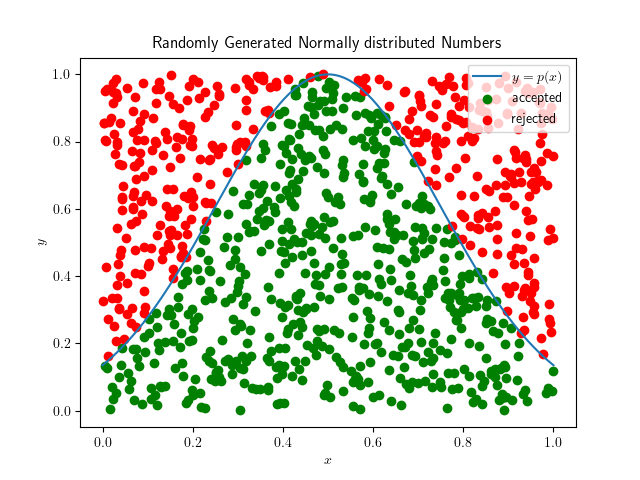
\includegraphics[scale=0.6]{randomly_generated_normally_distributed.png}
        \caption{Randomly generated points in \([0, 1)^2\). The green points under the curve are accepted and their \(x\) coordinates are normally distributed.}
        \label{fig:rng normal}
    \end{figure}

    For specific distributions it is possible to improve this process if instead of generating points in \([a, b)\times[0, 1)\) we generate points in some under some curve, \(q\) such that \(q(x) < p(x)\) for all \(x \in [a, b)\).
    A common way to do this for a normal distribution is with the Ziggurat distribution which uses a sort of staircase going up the side of the normal distribution.
    This speeds up the algorithm by decreasing the number of points that need to be rejected.
    
    \subsection{Applications of Monte Carlo Methods}
    \subsubsection{High Dimensional Integrals}
    The integration methods that we have discussed are very slow for high dimensional integral.
    In general if we want to form
    \[\int_V \dd[D]{r} f(\vv{r})\]
    for \(D \gg 1\) then if moderate accuracy is acceptable, or if \(V\) is a complicated shape, then Monte Carlo integration may be the best algorithm.
    This works by the following approximation:
    \[\int_V \dd[D]{r} f(\vv{r}) \approx V\expected{f} \pm V\sqrt{\frac{\expected{f^2} - \expected{f}}{N}}.\]
    Here \(\expected{\cdot}\) denotes the mean which we approximate by generating \(N\) points \(\{\vv{r_i}\} \subset V\) and then computing
    \[\expected{f} = \frac{1}{N}\sum_{i=1}^{N} f(\vv{r_i}), \qquad\text{and}\qquad \expected{f^2} = \frac{1}{N}\sum_{i=1}^{N} [f(\vv{r_i})]^2.\]
    The error here scales as \(1/\sqrt{N}\) so we need many points to achieve a good (three or four significant figures) level of accuracy.
    The accuracy of \(\num{e-12}\) or better that we achieved with other deterministic algorithms is simply not possible as it would take an infeasible \(\num{e24}\) points to reach this level of accuracy.
    
    This method of integration was applied to the integral
    \[\int_{\reals^2}e^{-(x^2 + y^2)/2} \dd{S} = 2\pi.\]
    First we need a proper integral so we approximate limit our integration to some subset of the plane ,\([-a, a]^2\), choosing \(a\) such that \(e^{-a^2}\) is sufficiently close to zero that we can ignore it.
    We then apply the Monte Carlo method with \(N = \num{e6}\).
    The values we got from repeated calculations where \(6.26833\), \(6.27074\), and \(6.28916\).
    Comparing these to the correct value of \(2\pi = 6.28319\) we see that the accuracy is approximately \(\pm0.01\).
    Note that in reality a deterministic method could still be applied here but if we took the same function in ten dimensions then a Monte Carlo method would be the best we can do.
    
    \subsection{Stochastic Computer Models}
    Suppose we have a case of diffusion with sinks but we don't know where the sinks are.
    We can model this situation with the \gls{pde}
    \[\pdv{u}{t} = \pdv[2]{u}{x} - \sum_{i}S(x - x_i)\]
    where \(S\) is some sink function and \(\{x_i\}\) are the positions of the sinks.
    We can still get a rough idea of what would happen by solving the \gls{pde} multiple times with a randomly generated set, \(\{x_i\}\), of sink positions.
    
    \subsection{Error Propagation}
    The standard way to propagate errors for \(y = y(x_1, x_2, \dotsc)\) where we know the standard deviation of the means (also known as the standard errors), \(\sigma_{\bar{x}_1}, \sigma_{\bar{x}_2}, \dotsc\), is to apply the formula
    \[\sigma_{\bar{y}} = \sqrt{\sigma_{\bar{x}_1}\abs{\pdv{y}{x_1}}^2 + \sigma_{\bar{x}_2}\abs{\pdv{y}{x_2}}^2 + \dotsb}.\]
    However this doesn't work if we don't have an explicit form for \(y\), or if \(y\) is a particularly complicated function.
    For example, \(y\) may be the solution to some \gls{pde}.
    Instead we use a Monte Carlo method of error propagation as follows:
    \begin{itemize}
        \item Generate parameters, \(x_i\), from a normal distribution with standard deviation \(\sigma_{\bar{x}_i}\).
        \item Calculate \(y\) numerically and store the value of \(y\).
        \item Repeat \(N\) times and get a set of values \(\{y_i\}\) for each set of \(x\) values.
        \item The standard error on the mean is
        \[\sigma_{\bar{y}} = \sqrt{\frac{1}{N - 1} \sum_{i}(y_i - \bar{y})},\qquad\text{where}\qquad \bar{y} = \frac{1}{N}\sum_i y_i.\]
    \end{itemize}
    
    \subsection{Random Numbers in \texorpdfstring{\lstinline|numpy|}{numpy}.}
    The correct way to generate random numbers in \lstinline|numpy| is to create a \lstinline|Generator| object by doing
    \begin{lstlisting}
    import numpy as np
    rng = np.random.default_rng()
    \end{lstlisting}
    If a specific seed is wanted then this can be passed as an argument as \lstinline|np.random.default_rng(seed)|.
    This can then be used to create various random numbers:
    \begin{itemize}
        \item \lstinline|rng.random()|  -- Generate a uniformly distributed random number in \([0, 1)\).
        This can then be mapped to \([a, b)\) by doing \lstinline|rng.random() * (b - a) + a|.
        \item \lstinline|rng.random(size)| -- Generate an array of length \lstinline|size| of uniformly distributed random numbers in \([0, 1)\).
        \item \lstinline|rng.normal(loc, scale, size)| -- Generate an array of length \lstinline|size| of normally distributed random numbers with mean \lstinline|loc| and standard deviation \lstinline|scale|.
        \item \lstinline|rng.binomial(n, p, size)| -- Generate an array of length \lstinline|size| of binomially distributed random numbers with \lstinline|n| trials and a probability of success \lstinline|p|.
    \end{itemize}
    There are many other distributions that \lstinline|numpy| can draw from and there are many other \glspl{rng} than the default.
    However for most uses the default is fine.
    
    \section{Signal Processing}
    \subsection{Sampling}
    A signal can be though of as function, \(f\colon\reals\to\reals\).
    A continuous signal, such as audio, cannot be handled directly by a computer.
    It must first be digitised.
    The simplest way to do this is to sample the signal at a constant sampling frequency, \(f_S\), storing the value of the function, \(f(t_n)\), at regularly spaced times, \(t_n = t_0 + n/f_S\).
    This turns an analogue signal into a digitised one consisting of two arrays, one containing the values of \(t_n\) and another containing the values of \(f(t_n)\).
    
    The sampling rate, \(f_S\), is important for the quality of the digitising since if the sampling rate is too low then information will be lost.
    Some values that may be considered normal sample rates in different scenarios are given in table~\ref{tab:sample rates}.
    \begin{table}[ht]
        \centering
        \begin{tabular}{ll}\hline
            System & \(f_S\)\\\hline
            Digital voltmeter & \SI{3}{\hertz}\\
            CD audio & \SI{44100}{\hertz}\\
            Digital oscilloscope & \SIrange{10}{1000}{\mega\hertz}\\
            Fastest digital oscilloscope (costs \pounds 1M) & \SI{240}{\giga\hertz}\\\hline
        \end{tabular}
        \caption{Sampling rates in a variety of scenarios.}
        \label{tab:sample rates}
    \end{table}
    \subsubsection{Aliasing and Nyquist Frequency}
    When we digitally sample a continuous signal we typically lose information.
    For example if we sample a sine wave, \(\sin(tf_{\text{signal}})\), of frequency \(f_\text{signal}\), at a rate \(f_S\) then a sine wave of frequency \(f_\text{signal}\), this is known as aliasing.
    An example of this is plotted in figure~\ref{fig:aliasing}
    \begin{figure}[ht]
        \centering
        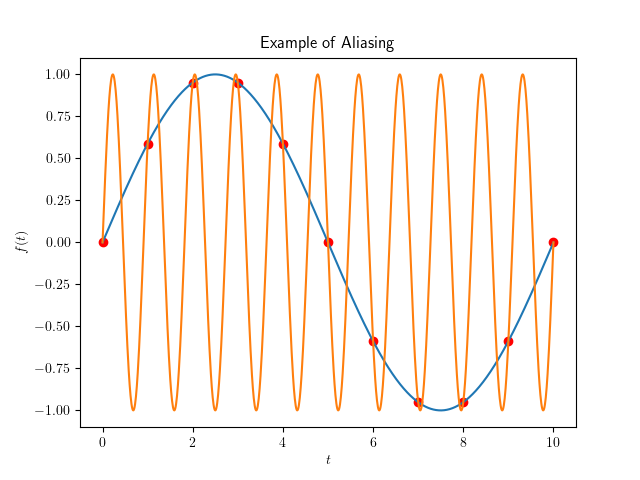
\includegraphics[scale=0.6]{aliasing.png}
        \caption{An example of aliasing of two sine waves.}
        \label{fig:aliasing}
    \end{figure}
    The sampling theorem states that a signal can be perfectly reproduced so long as \(f_\text{signal} < f_S/2\).
    If this is the case then the lower frequency signal in the example is the only one allowed.
    If this isn't the case then both signals are valid, most algorithms assume this to be true so will reconstruct the lower frequency signal given the sampled data.
    The frequency \(f_S/2\) is called the Nyquist frequency.
    For a signal other than a pure sine wave if we decompose it into a Fourier series then this applies to all terms with \(f_\text{signal}\) being the highest frequency present.
    
    \subsection{Fourier Transforms}
    Let \(f\colon\reals\to\complex\).
    The Fourier transform of \(f\) is defined as
    \[\FT[f](\omega) = \tilde{f}(\omega) = \int_{-\infty}^{\infty} \dd{t} f(t)e^{i\omega t}.\]
    The inverse Fourier transform is defined as
    \[\FT^{-1}[\tilde{f}](t) = f(t) = \frac{1}{2\pi} \int_{-\infty}^{\infty} \dd{\omega} \tilde{f}(\omega) e^{-i\omega t}.\]
    If \(f\colon\reals\to\reals\) then
    \[\tilde{f}(\omega) = \tilde{f}^*(-\omega).\]
    In general \(\tilde{f}\colon\reals\to\complex\) even if \(f\colon\reals\to\reals\).
    \(|\tilde{f}(\omega)|\) represents the amplitude of the Fourier mode with frequency \(\omega\) and \(\arg(\tilde{f}(\omega))\) represents the phase of the mode.
    \(|\tilde{f}(\omega)|^2\) is called the power series and represents the amount of power concentrated in the Fourier mode with frequency \(\omega\).
    For example when doing NMR molecular bonds are vibrated and the power series is plotted as this shows the frequencies at which the majority of vibration is happening and this is related to the molecular structure.
    \begin{figure}[ht]
        \centering
        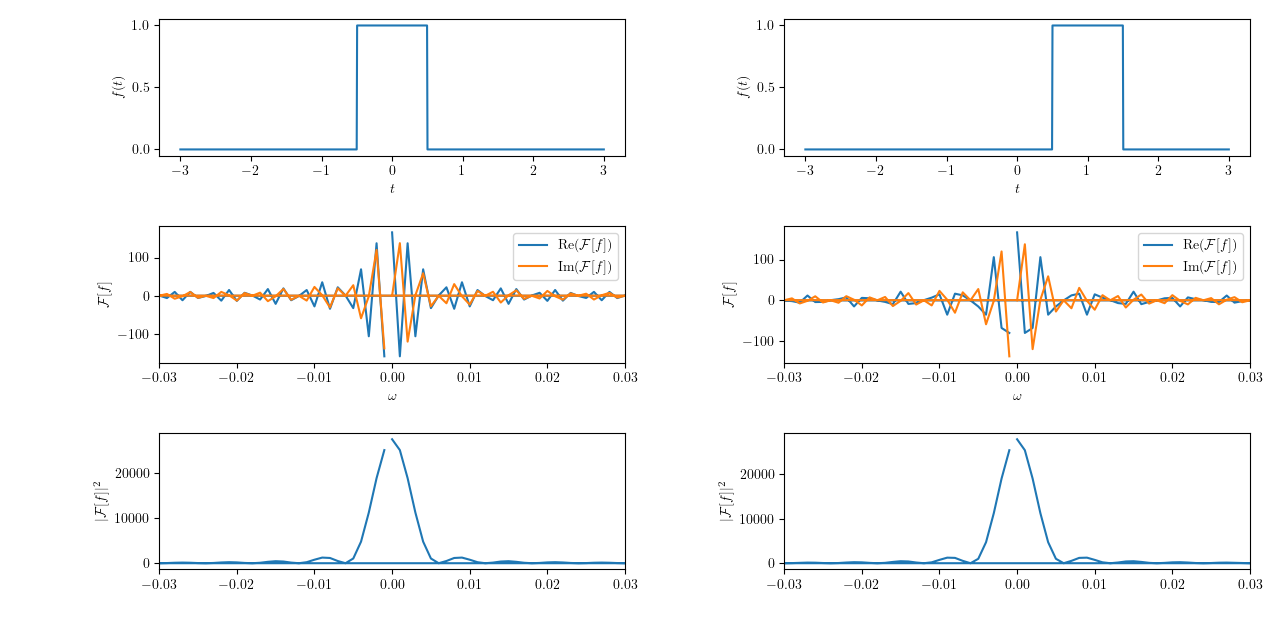
\includegraphics[scale=0.4]{FT_example.png}
        \caption{The Fourier transform of two top hats of the same width and height but different positions. Notice that the Fourier transforms are different but the power series are the same.}
        \label{fig:FT example}
    \end{figure}

    \subsubsection{Discrete Fourier Transform}
    As usual computers cannot deal with continuous functions so we discretise.
    The \acrfull{dft} is defined by
    \[\tilde{f}_k = \sum_{j=0}^{N-1} f_je^{2\pi jk/N}\]
    where \(f_j = f(t_j)\) is the function sampled at the \(j\)th point.
    The inverse of this is then
    \[f_j = \frac{1}{N}\sum_{k=0}^{N-1}\tilde{f}_ke^{-i2\pi jk/N}.\]
    Notice the similarity with the continuous Fourier transform.
    In both there is a normalisation factor in the inverse Fourier transform (\(1/2\pi\) in the continuous case and \(1/N\) in the discrete version).
    Similarly the sign in exponential of the forward and backwards transformations are always different.
    The discrete transform, like the continuous case, is Hermitian, meaning \(\tilde{f}_k = \tilde{f}_{-k}^*\) if \(f_j\in\reals\) for all \(j\).
    \begin{figure}[ht]
        \centering
        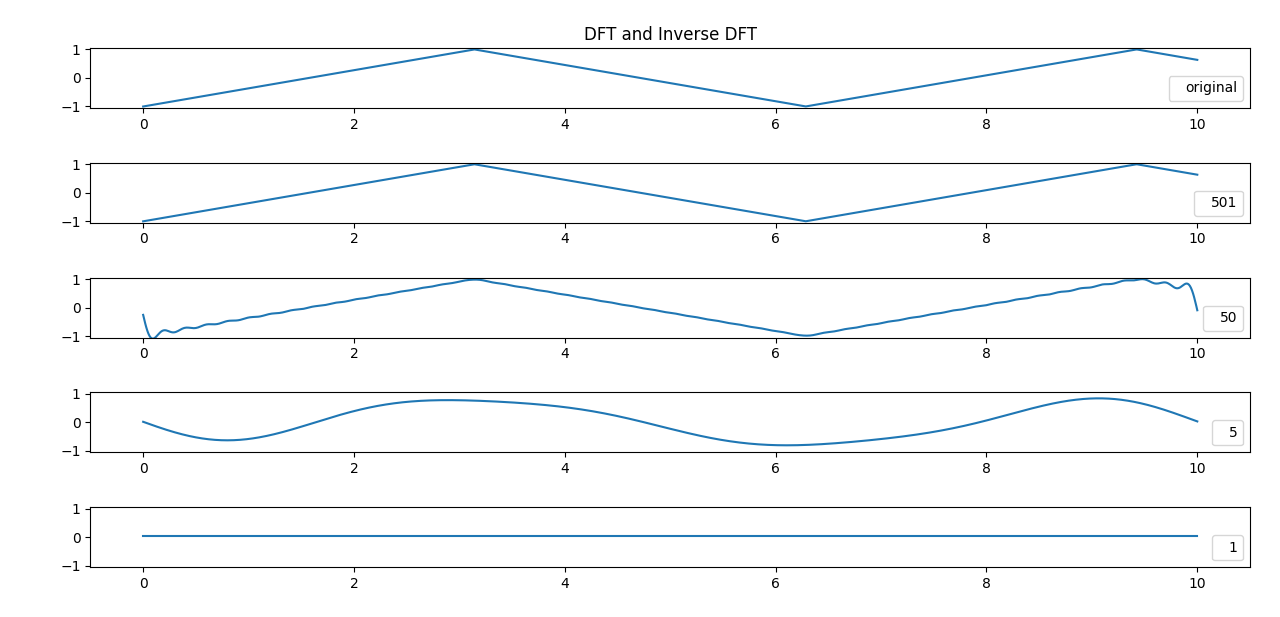
\includegraphics[scale=0.4]{dft.png}
        \caption{The \gls{dft} of a triangle wave plotted for various values of \(N\).}
    \end{figure}

    \subsubsection{Fast Fourier Transform}
    The naive implementation of the \gls{dft} is \(\order{N^2}\).
    Fortunately there is an implementation, known as the \acrfull{fft}, which is \(\order{N\log N}\).
    It is implemented using the following:
    \begin{align*}
        \tilde{f}_k &= \sum_{j=0}^{N-1} f_je^{i2\pi jk/N}\\
        &= \sum_{j=0}^{N/2-1} f_{2j} e^{i2\pi(2j)k/N} + \sum_{j=0}^{N/2-1} f_{2j+1} e^{i2\pi(2j+1)k/N}\\
        &= \sum_{j=0}^{N/2-1} f_{2j}e^{i2\pi jk/(N/2)} + e^{i2\pi k/N}\sum_{j=0}^{N/2-1} f_{2j+1}e^{i2\pi jk/(N/2)}\\
        &= \FT[f_j~\text{where}~j~\text{is even}] + e^{i2\pi k/N} \FT[f_j~\text{where}~j~\text{is odd}]
    \end{align*}
    So we see that we can split the \gls{dft} into two \glspl{dft} of half the size.
    This improves the efficiency and by padding the array with zeros so that \(N = 2^n\) for some \(n\in\naturals\) we can keep splitting the \gls{dft} until we are taking the \gls{dft} of single elements, which is a simple matter of multiplication by an exponential.
    
    One application of \gls{fft} is filtering signals.
    Suppose we have a signal and it has some sort of noise included.
    If we know that the information in the signal is concentrated at lower frequencies then we can filter out higher frequencies by Fourier transforming, setting higher frequency terms to zero, and transforming back.
    This is called a \gls{lpf} as only low frequency terms make it through.
    This is shown in figure~\ref{fig:lpf}.
    The initial signal in this case was a pure sine wave.
    Notice that the filtered signal isn't quite a pure sine wave as there were some frequencies associated with noise that where kept.
    This can be seen in the plot of the Fourier transformed signal.
    In the case of a signal that is a pure sine wave, or a sum of a small number of sine waves, we can pick out exactly the frequencies of the sine waves present and reconstruct the signal exactly without noise.
    In the case of a real life signal like audio there are simply too many important frequencies for this to work.
    Another improvement that can be made is instead of abruptly setting all high frequencies to zero the amplitude can be gradually decreased which is more effective.
    Filters are also often implemented in hardware as well as being added in post to a signal.
    For example a simple resistor--capacitor circuit acts as a \gls{lpf} and a resistor--inductor circuit acts as a \gls{hpf}.
    A \gls{lpf} and \gls{hpf} can be combined to create a bandwidth filter which only permits frequencies higher than the minimum frequency of the \gls{hpf} and lower than the maximum frequency of the \gls{hpf}.
    This can be used to remove noise from both sides of a signal's peak frequency.
    \begin{figure}[ht]
        \centering
        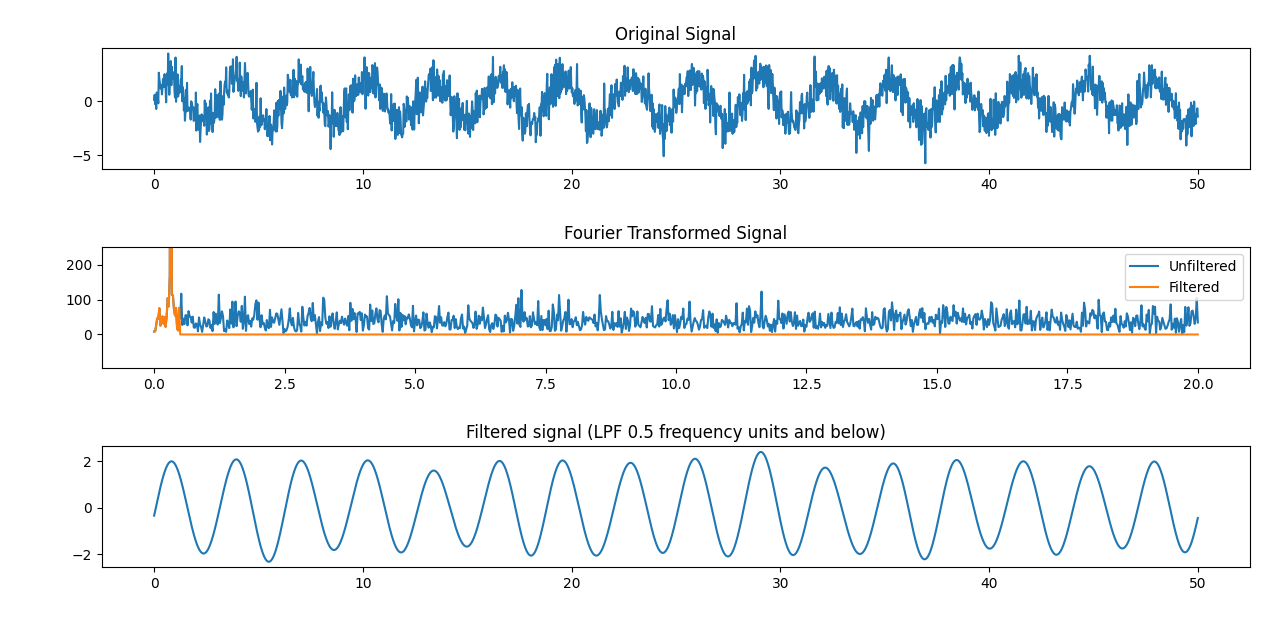
\includegraphics[scale=0.4]{lpf.png}
        \caption{Low pass filter applied to a noisy signal.}
        \label{fig:lpf}
    \end{figure}

    \subsubsection{Convolution/Deconvolution}
    The convolution of \(f, g\colon\reals\to\complex\) is defined as
    \[(f\convolution g)(t) = \int_{-\infty}^{\infty} f(\tau)g(t - \tau)\dd{\tau}.\]
    Or in the discrete case
    \[(f\convolution g)_n = \sum_{m=0}^{N-1}f_mg_{n-m}.\]
    The naive implementation of this is \(\order{N^2}\).
    The convolution theorem states that
    \[\FT[f\convolution g] = \FT[f]\FT[g].\]
    Since the Fourier transform can be applied as \(\order{N\log N}\) using the \gls{fft} this means that so too can convolutions.
    
    A related concept is the auto-correlation of a function, \(f\colon\reals\to\complex\):
    \[A(t) = \int_{-\infty}^{\infty} f(\tau + t)f^*(\tau)\dd{\tau}\]
    or in the discrete case
    \[A_n = \sum_{m=0}^{N-1}f_mf_{m+n}.\]
    This can also be computed with Fourier transforms:
    \[A_n = \FT^{-1}[\abs{\FT[f]}^2].\]
    We assumed here that \(f\) and \(g\) are periodic so \(f_{-n} = f_{N-n}\), and similarly for \(g\).
    If we don't want them to be periodic then we have to pad the ends of the arrays with zeros over the whole range of interest.
    
    \subsubsection{Multi-Dimensional Fourier Transforms}
    In two dimensions the \gls{dft} of \(f\colon\reals^2\to\complex\) is
    \begin{align*}
        \tilde{f}_{k_1k_2} &= \sum_{j_1 = 0}^{N_1 - 1} \sum_{j_2 = 0}^{N_2 - 1} f_{j_1j_2}e^{i2\pi j_1k_1/N_1}e^{i2\pi j_2k_2/N_2}\\
        &= \FT_1[\FT_2[f_{j_1j_2}]]
    \end{align*}
    where \(\FT_i\) is the one-dimensional Fourier transform on the \(i\)th index of \(f\).
    The inverse is then
    \begin{align*}
        f_{j_1j_2} &= \frac{1}{N_1N_2}\sum_{k_1 = 0}^{N_1 - 1} \sum_{k_2 = 0}^{N_2 - 1} \tilde{f}_{k_1k_2}e^{-i2\pi j_1k_1/N_1}e^{-i2\pi j_2k_2/N_2}\\
        &= \FT_2[\FT_1[\tilde{f}_{k_1k_2}]].
    \end{align*}
    The generalisation to \(D\) dimensions is
    \begin{align*}
        \tilde{f}_{k_1\dotso k_D} &= \sum_{j_1 = 0}^{N_1 - 1} \dotsb \sum_{j_D = 0}^{N_D - 1} f_{j_1\dotso j_D}\prod_{m=1}^{D} e^{i2\pi j_mk_m/N_m}\\
        &= (\FT_1\circ \dotsb \circ \FT_D)[f_{j_1\dotso j_D}]\\
        &= \FT_1[\dotsb \FT_D[f_{j_1\dotso j_D}]]\\
        &= \prod_{m=1}^{D}\FT_{D-m}[f_{j_1\dotso j_D}]
    \end{align*}
    where \(\circ\) represents function composition.
    The inverse is generalised similarly.
    
    This has many applications, particularly in image processing.
    For example applying a \gls{lpf} to an image to remove high frequency data can compress the image without removing the important data.
    Image deconvolution (reversing a convolution using the convolution theorem) can be used to apply other filters including removing diffraction and other artefacts from images.
    
    \section{Minimisation}
    \subsection{General Problem}
    The general problem that we want to solve with minimisation is finding the minimum of a function, \(y\colon\reals^n\to\reals\) in some region \(V\subseteq\reals^n\).
    The naive approach is to calculate the roots of \(\grad y\).
    However this is often difficult/impossible and even if we do succeed it doesn't allow us to tell the difference between minima and maxima and it can also lead to problems with discontinuity.
    
    Note that we will talk in this section about minimising \(y\) but maximising \(y \) is the same as minimising \(-y\) so all of these algorithms can be used to maximise a function as well.
    
    Three problems that we often have when trying to minimise a function are
    \begin{itemize}
        \item Multiple minima
        \item Local (easy) vs. global (very hard) minima
        \item Minima at boundaries
    \end{itemize}
    
    \subsection{One-Dimensional Golden Section}
    Recall the bisection algorithm used for root finding, discussed in section~\ref{sec:bisection method}.
    The root is found by the following algorithm:
    \begin{itemize}
        \item Bracket the root in \([a, b]\) and set \(c = (a + b)/2\).
        \item Choose \([a, c]\) if \(y(a)y(c) < 0\) else choose \([c, b]\).
        \item Make this the new bracket and repeat until sufficient accuracy is reached.
    \end{itemize}
    The golden section algorithm for finding minima is similar to this:
    \begin{itemize}
        \item Select three points, \(a\), \(b\), and \(c\) with \(a < c < b\) such that \(y(c) < y(a)\) and \(y(c) < y(b)\).
        This guarantees that there is a minimum in \([a, c]\) if \(y\) is continuous.
        \item Choose a new point, \(x\in[a, b]\).
        \item If \(y(c) < y(x)\) then set \(b\) to \(x\) else set \(a\) to \(c\) and \(c\) to \(x\).
        \item Iterate until \(\abs{c - x} < \varepsilon\) for some pre-decided accuracy, \(\varepsilon\).
    \end{itemize}
    The best choice for \(x\) depends on which of two scenarios occurs.
    If \(x \in [a, c]\) then choose
    \[x = b - \frac{b - a}{\varphi},\]
    and if \(x\in [c, b]\) then choose
    \[x = a + \frac{b - a}{\varphi}\]
    where 
    \[\varphi = \frac{1 + \sqrt{5}}{2} \approx 1.6180\]
    is the golden ratio.
    This choice will give the fastest convergence to the minimum.
    
    \subsection{One-Dimensional Parabolic Interpolation}
    As with the golden section algorithm we start with points \(a\), \(b\), and \(c\) bracketing the minimum.
    We fit a parabola to these points.
    Assuming \(y\) is analytic then near the minimum, \(x_0\), we can express \(y\) to second order as
    \[y(x) \approx y(x_0) + \frac{1}{2}y''(x_0)(x - x_0)^2\]
    where we have used that \(y'(x_0) = 0\).
    We can find the minimum of this parabola fairly easily using
    \[x_0  = c - \frac{\frac{1}{2}(c - a)^2[y(c) - y(b)] - (c - b)^2[y(c) - y(a)]}{(c - a)[y(c) - y(b)] - (c - b)[y(c) - y(a)]}.\]
    We can repeat the algorithm choosing \(c = x_0\) until the desired accuracy is achieved.
    
    This converges faster than the golden section method \emph{if} it converges.
    However this algorithm will not converge if it is too far from a minima and it will also converge to maxima.
    The best solution is to use Brent's method, which is similar to the root finding method of the same name, which attempts parabolic interpolation at each step and reverts to golden section when necessary.
    This can be accessed from \lstinline|scipy| using
    \begin{lstlisting}
    scipy.optimize.minimize_scalar(fun, bracket, bounds=None, args=(), method="brent", too=None, options=None)
    \end{lstlisting}
    where \lstinline|fun| is a callable that returns a real number which this method will minimise with respect to its first argument.
    The default is \lstinline|method="brent"| but it is also possible to use \lstinline|method="golden"| or \lstinline|method="bounded"| to use the golden sections method.
    
    Another useful function for finding the bracketing is
    \begin{lstlisting}
    scipy.optimize.bracket(function, xa=0, xb=1, args=(), grow_limit=110, maxiter=1000)
    \end{lstlisting}
    which will return a bracketing, \lstinline|(a, b)|, suitable for use as the interval \([a, b]\) as defined above.
    However it is better to set the bracketing manually if possible as it is possible to get a tighter bracket and hence faster convergence.
    It is also possible that this \lstinline|bracket| method will fail.
    
    \subsection{Multi-Dimensional Minimisation}
    The Golden sections method doesn't generalise to more dimensions.
    Parabolic interpolation does. 
    It often requires us to calculate the Hessian matrix,
    \[H_{ij} = \pdvsec{f}{x_j}{x_i},\]
    which can be computed numerically by some routines.
    
    \subsection{Conjugate Directions}
    This algorithm allows us to use one-dimensional minimisation to minimise a \(D\)-dimensional function:
    \begin{itemize}
        \item Choose a start point, \(\vv{x_\text{start}}\in\reals^D\).
        \item Choose a direction, \(\vv{n}\in\reals^D\).
        \item Let \(\vv{x} = \vv{x_\text{start}} + \lambda\vv{n}\).
        \item Minimise \(y(\vv{x})\) with respect to \(\lambda\).
        \item Choose another direction and iterate from the second step choosing the point \(\vv{x}\) which minimised \(y(\vv{x})\) along \(\vv{x_\text{start}} + \lambda\vv{n}\) as the new start point.
    \end{itemize}
    The most obvious choice of \(\vv{n}\) is as successive basis vectors.
    This will work but is often not the fastest choice.
    
    \subsubsection{Powell's Method}
    Powell's method gives a way of choosing the directions, \(\vh{n_i}\), for fast convergence:
    \begin{itemize}
        \item Initialise the start point, \(\vv{x_0}\in\reals^D\),
        \item Initialise \(\vh{n}\vv{_i} = \ve{i}\) for \(i = 1, \dotsc, D\).
        \item For \(i = 1, \dotsc, D\) calculate \(\vv{x_i} = \vv{x_{i-1}} + \lambda\vv{n_i}\) where \(\lambda\) is chosen such that \(y(\vv{x})\) is minimised with respect to \(\lambda\).
        \item For \(i = 1, \dotsc, D-1\) set \(\vv{n_i} = \vv{n_{i+1}}\).
        \item Set \(\vv{n_D} = \vv{x_D} - \vv{x_0}\).
        \item Move \(\vv{x_D}\) to the minimum along the direction \(\vv{n_D}\) and call this new point \(\vv{x_0}\).
        \item Repeat until the distance moved is larger than \(\varepsilon\).
    \end{itemize}
    If \(y\) is parabolic then the line parallel to \(\vv{n_D}\) crossing through \(\vv{x_0}\) as defined after one run of the algorithm will intersect the minimum.
    
    \subsection{Monte Carlo Minimisation}
    The naive Monte-Carlo approach is to choose \(N\) points at random in \(\reals^D\) and compute \(y(\vv{x})\) at each point and then choose the lowest of these as the minimum.
    Clearly this is terrible.
    This method is \(\order{N}\) but we need \(N\) to be unfeasibly large to have good accuracy compared to other methods.
    
    A better approach is to start with random points and then do a deterministic (non-Monte Carlo) method to find a local minimum.
    Repeat this multiple times and select the lowest minimum.
    
    A third more complicated method is known as simulated annealing.
    The name comes from the idea that a system that is cooled slowly will settle into a minimum energy scenario.
    The slower the material is cooled the more likely the system is to find a global minima.
    This is the difference between crystals and glasses.
    The algorithm to find the minima by simulated annealing is as follows:
    \begin{itemize}
        \item Set the starting point, \(\vv{x}\), and `temperature', \(T\).
        \item Calculate the `energy', \(E = y(\vv{x})\).
        \item Update \(\vv{x}\) to a new position, \(\vv{x'}\).
        The move should be small.
        \item Calculate the new energy, \(E' = y(\vv{x'})\).
        \item Accept the new position with probability
        \[\min\left(1, e^{-(E' - E)/T}\right).\]
        \begin{itemize}
            \item If the point is rejected start again with a different \(\vv{x'}\).
            \item If the point is accepted update \(E\) to \(E'\) and \(\vv{x}\) to \(\vv{x'}\), decrease \(T\) and iterate.
        \end{itemize}
    \end{itemize}
    This method requires a lot of experimentation to find the bet way to update \(\vv{x}\) and the best way to decrease \(T\), known as the cooling protocol.
    This method can be very efficient for functions with many local minima if the cooling protocol and update scheme are well chosen.
    
    \subsection{Multi-Dimensional Minimisation with SciPy}
    The following will minimise a callable, \lstinline|fun|, with respect to its first argument:
    \begin{lstlisting}
    scipy.optimize.minimize(fun, x0, args=(), method=None, jac=None, hess=None, hessp=None, bounds=None, constraints=(), tol=None, callback=None, options=None)
    \end{lstlisting}
    There are many choices for \lstinline|method| including \lstinline|method="powell"|.
    For finding global minima have a look at the following two functions
    \begin{lstlisting}
    scipy.optimize.basinhopping(...)
    scipy.optimize.dual_annealing(...)
    \end{lstlisting}
    For curve fitting, which often uses minimisation techniques, there exists curve fitting functions with inbuilt minimisation such as
    \begin{lstlisting}
    scipy.optimize.curve_fit(...)   # for non-linear fitting
    scipy.optimize.lsq_linear(...)  # for linear multi-dimensional fitting
    numpy.polyfit(...)              # for polynomial fitting
    \end{lstlisting}
    
    \section{Statistical Data Analysis}
    There are two broad categories of problems that we may wish to solve:
    \begin{itemize}
        \item Model independent problems -- descriptive statistics such as calculating the mean/variance of a set of data or comparing two datasets.
        These are numerically simple problems and we will focus on the second type of problems here.
        \item Model dependent problems -- testing models and comparing to see which fits better, parameter estimation and error estimation.
    \end{itemize}
    
    \subsection{Model Based Statistics}
    The general problem is given a vector of experimental data, \(\vv{D}\), which could be from an actual experiment or the result of a computer simulation, we need to find a model that fits.
    Once we have a model it will typically have parameters, \(\vv{\vartheta}\), we need to calculate the modelled data, \(\vv{d}\), and compare to the true data, \(\vv{D}\), to estimate the values of the parameters.
    The model could be a simple function of the form \(\vv{d} = \vv{f}(\vv{\vartheta})\), or it could be a complicated computer simulation.
    The model must include a measurement of errors since the model encodes the physics that we care about and there is a measuring process so there must be some error.
    
    We will use a working example where \(\vv{D} = \{(x_i, y_i)\st i =1, \dotsc, N\}\) which we will try to fit to a linear model, \(y = A + Bx + \text{err}\) where \(\text{err}_i\) is the error on the measurement of \(y_i\).
    We will assume that \(\text{err}\) is normally distributed with mean \(0\) and variance \(\sigma^2\).
    The parameters in this case are \(\vv{\vartheta} = [A, B, \sigma]\).
    We will generate \(\vv{D}\) from the model with \(A = 0\), \(B = 1\), \(\sigma = 1\), and \(N = 10\).
    We will then use this to test various methods.
    This generated data set is plotted in figure~\ref{fig:data set}
    \begin{figure}[ht]
        \centering
        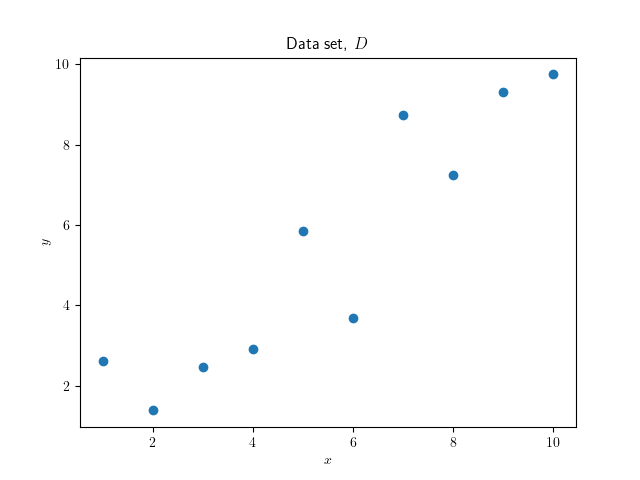
\includegraphics[scale=0.6]{data_set.png}
        \caption{The data set we will use to test our statistical models.
        This data set was generated as \(y = x + \text{err}\) where \(\text{err}_i\sim\mathcal{N}(\mu=0, \sigma^2=1)\).}
    \end{figure}
    
    \subsection{Maximum Likelihood Method}
    The likelihood of a set of data, \(\vv{D}\), given a particular model, \(M\), which is in general a function of some parameters, \(\vv{\vartheta}\), is the probability that we would observe the data, \(\vv{D}\), from that model, with that set of parameters.
    This is written \(L = P(\vv{D}\st\vv{\vartheta})\).
    This can be used through the \gls{mlm} which, as the name suggests, looks for a set of parameters that maximises \(L\).
    These are the so called `best fit' parameters.
    In general the form of \(L\) will be quite complicated and we use numerical methods, discussed in the last section, to maximise \(L\) (or minimise \(-L\)).
    
    For our working example
    \[L = P(\{(x_i, y_i)\}\st A, B, \sigma) = \prod_{i=1}^{N} \frac{1}{\sigma^2\sqrt{2\pi}}\exp\left[-\frac{1}{2\sigma^2}(y_i - A - Bx_i)^2\right].\]
    This assumes that each data point is independent of the others and we use the fact that \(\text{err}_i = y_i - A - Bx_i\) and then we simply use the product of independent terms as the total probability.
    Rearranging the likelihood we get
    \[\ln L = \text{const} - \frac{1}{2\sigma^2}\sum_{i=1}^{N} (y_i - A - Bx_i)^2\]
    So we see that maximising \(L\) is the same as minimising
    \[S^2 = \sum_{i=1}^{N}(y_i - A - Bx_i)^2.\]
    From this we can derive the usual formula for least squares regression.
    If we were using something more complicated than a linear regression we would get a different result.
    In general least squares regression, that is minimising
    \[S^2 = \sum_{i=1}^{N} (y_i - f(x_i))^2\]
    where the model used is \(y = f(x)\), is equivalent to the \gls{mlm} if \(\text{err}\sim\mathcal{N}(0, \sigma^2)\), but if this isn't the case then the two methods will gives different results.
    
    \begin{figure}[ht]
        \centering
        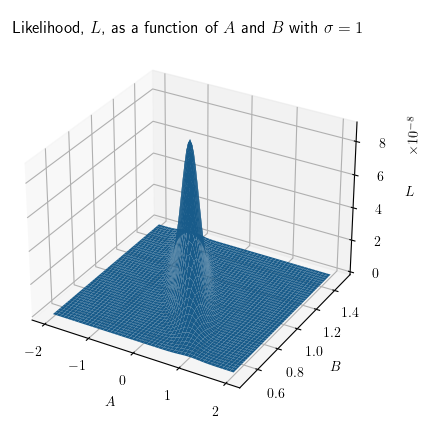
\includegraphics[scale=0.75]{likelihood.png}
        \caption{The likelihood, \(L\), of our working example with \(\sigma\) held constant at 1 to ease visualisation. Notice the maximum likelihood is at approximately \(A = 0\) and \(B = 1\). The actual likelihood values aren't important, just the location of the maximum. The peak is at \(A = -0.12244897959183687\) and \(B = 1.010204081632653\)}
    \end{figure}
    \begin{figure}[ht]
        \centering
        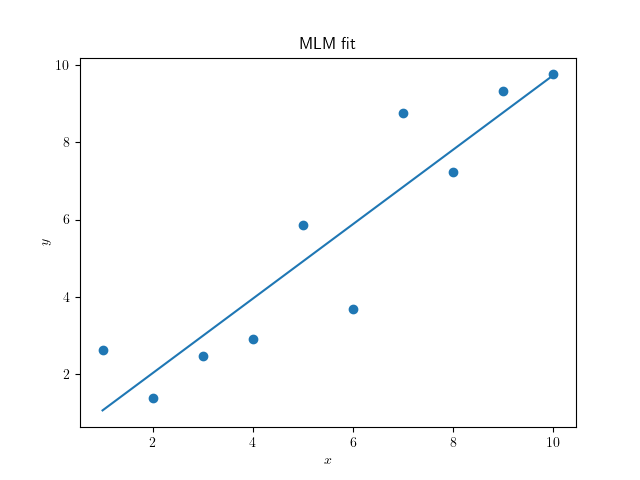
\includegraphics[scale=0.6]{mlm_fit.png}
        \caption{The fit line found by \gls{mlm} for our working example. This estimates \(A = 0.11041424234592867\) and  \(B = 0.9622627030632674\).}
    \end{figure}

    \subsubsection{Numerical methods for MLM}
    For more complicated (non-linear) models we have to find the best fit parameters by numerically maximising the likelihood.
    In practice we always work with \(\ln L\), not \(L\), as \(L\) is often unreasonably small, for example in our working example the maximum likelihood is about \num{8e-8}, so \(\ln L\) peaks at \(-16.3\).
    Using values that are larger (in magnitude) avoids a lot of floating point error and rounding issues.
    The plot of \(\ln L\) is also less steep.
    \begin{figure}[ht]
        \centering
        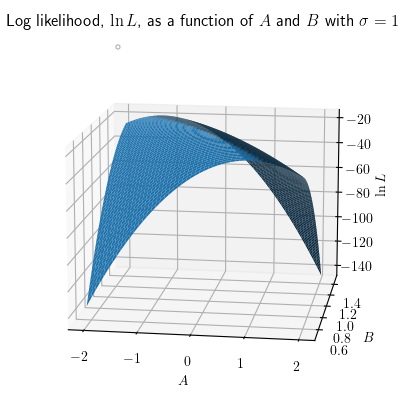
\includegraphics[scale=0.75]{log_likelihood}
        \caption{The log likelihood, \(\ln L\), of our working example with \(\sigma\) held constant at 1 to ease visualisation. Notice that the maximum is still at approximately \(A = 0\) and \(B = 1\). The magnitude of the log likelihood is on the order of 10 near the maximum, as opposed to the \num{e-8} scale used for \(L\).}
    \end{figure}
    Since this method requires us to maximise a function it has all the same issues as any other maximisation problem such as finding local vs. global maxima.
    We are in general only interested in the global maximum.
    To ensure we find it we try a Monte Carlo method where we choose many different start points and find the maximum with some maximisation routine and then choose the largest maximum found.
    
    For cases where the probability distribution is well understood and the model is not too complicated there are often algorithms designed for that particular problem, least squares is one such algorithm.
    
    \subsection{Bayesian Inference}
    We want to find \(P(\vv{\vartheta}\st \vv{D})\), that is given the data what is the probability that a given set of parameters is correct?
    We do this using Bayes' theorem:
    \[P(\vv{\vartheta}\st\vv{D}) = \frac{P(\vv{D}\st\vv{\vartheta}) P(\vv{\vartheta})}{P(\vv{D})}.\]
    In this context \(P(\vv{\vartheta}\st\vv{D})\) is referred to as the posterior distribution, \(P(\vv{D}\st\vv{\vartheta})\) is the likelihood, given by the model, \(P(\vv{\vartheta})\) is the prior distribution which we choose as a sensible guess, finally \(P(\vv{D})\) can often be ignored as it is simply a normalisation factor and is not important as we are interested in looking for when \(P(\vv{\vartheta}\st\vv{D})\) is maximised.
    
    If we choose a uniform prior, where \(P(\vv{\vartheta}) = \text{const}\) for all \(\vv{\vartheta}\) in a sensible range, then \(P(\vv{\vartheta}\st\vv{D})\propto P(\vv{D}\st\vv{\vartheta})\) and Bayesian inference is equivalent to \gls{mlm}.
    
    When choosing a prior we should, if we don't have any other information, choose a uniform prior.
    If we have some information, say posteriors from previous experiments, then we should use these to inform our new priors.
    This is nice as it allows us to combine old and new data.
    
    Given \(P(\vv{\vartheta}\st\vv{D})\) we can calculate
    \begin{itemize}
        \item The average value of the parameters,
        \[\expected{\vv{\vartheta}} = \int \vv{\vartheta}P(\vv{\vartheta}\st \vv{D})\dd{\vv{\vartheta}}\]
        where \(\dd{\vv{\vartheta}} = \dd{\vartheta_1}\dd{\vartheta_2}\dotsm\).
        \item Higher moments, such as variance, which are defined similarly to the mean and are useful for calculating errors.
        \item The maximally probable parameters which maximise \(P(\vv{\vartheta}\st\vv{D})\).
        These values can then be used to estimate the true values.
    \end{itemize}
    
    However all of this assumes that we have a nice analytic expression for \(P(\vv{\vartheta}\st\vv{D})\).
    This is often not the case.
    The solution is, perhaps unsurprisingly at this point in this numerical recipes course, to use a numerical method.
    There are two such methods that are commonly used.
    The first is \gls{abc}, which is explained in the next section, and the second uses something called Monte Carlo Markov chain which won't be discussed here.
    
    \subsubsection{Approximate Bayesian Computation}
    The idea behind \gls{abc} is that we don't really need \(P(\vv{\vartheta}\st\vv{D})\), we can make do with a sample, \(\{\vv{\vartheta_i}\}\), generated from the same distribution behind \(P(\vv{\vartheta}\st\vv{D})\).
    We then calculate sample values, such as the mean, standard error, etc. which we then use as estimators of the relevant population statistics.
    We can also use this to get an estimate of the error on these values, although the error tends to zero as the number of data points grows so we can simply use a large sample \(\{\vv{\vartheta_i}\}\) and the error will be small.
    
    The \gls{abc} algorithm is
    \begin{itemize}
        \item Generate \(\vv{\vartheta}\) from the prior distribution, \(P(\vv{\vartheta})\).
        \item Simulate the model with parameters \(\vv{\vartheta}\), call the result \(\vv{d}\).
        \item Calculate the distance, \(\rho(\vv{D}, \vv{d})\), between the simulated and real data.
        \item Accept \(\vv{\vartheta}\) if \(\rho(\vv{D}, \vv{d}) < \varepsilon\) for some small \(\varepsilon > 0\), else start again.
        \item Repeat \(n\) times for some large \(n\) to get a sample, \(\{\vv{\vartheta_i}\}\) of size \(n\).
    \end{itemize}
    This is similar to the method for generating random numbers from a non-uniform distribution, see section~\ref{sec:non-uniform random numbers}.
    The outcome of the algorithm is a set of points, \(\{\vv{\vartheta_i}\}\), drawn from the sample \(P(\vv{\vartheta}\st\rho(\vv{D}, \vv{d}) < \varepsilon)\) which approximate a sample drawn from the posterior distribution, \(P(\vv{\vartheta}\st\vv{D})\).
    In the limit \(\varepsilon\to 0\) then it is exactly a sample drawn from the posterior distribution.
    
    The important thing for this algorithm is choosing \(\rho\) and \(\varepsilon\) so the algorithm has a non-zero acceptance rate but maintains accuracy.
    There are dedicated software packages for solving this problem.
    Note that distance needn't be Euclidean distance as this doesn't really mean anything physical in parameter space.
    For example in the one parameter case we may choose \(\rho(D, d) = \abs{D - d}\), \(\rho(D, d) = \abs{D} + \abs{d}\), \(\rho(D, d) = D^2 + d^2\), or \(\max\{\abs{D}, \abs{d}\}\).
    Once nice thing is that it turns out that the choice of priors is not actually that important, hence why a uniform distribution is often sufficient.
    
    \subsubsection{Errors via Bayesian Inference}
    The standard error on the mean of a single parameter is defined by
    \[\sigma_{\expected{\vartheta}} = \sqrt{\int(\vartheta - \expected{\vartheta})^2 P(\vartheta\st\vv{D})\dd{\vartheta}}.\]
    In \gls{abc} this becomes
    \[\sigma_{\expected{\vartheta}} = \sqrt{\frac{1}{n}\sum_i(\vartheta_i - \expected{\vartheta})^2}\]
    where we can estimate the mean as
    \[\expected{\vartheta} = \frac{1}{n}\sum_i \vartheta_i.\]
    We can also find the credibility interval, the interval \((\vartheta_-, \vartheta_+)\) such that
    \[\int_{\vartheta_-}^{\vartheta_+} P(\vartheta\st\vv{D})\dd{\vartheta} = X\]
    where \(X\) is the desired credibility.
    
    \subsubsection{Bayesian Model Selection}
    Suppose we have two models that give posterior distributions \(P_1(\vv{D}\st\vv{\vartheta})\) and \(P_2(\vv{D}\st\vv{\vartheta})\).
    We want to select the model that best fits the data.
    The idea is to generalise \gls{abc} so that as well as selecting parameters it also randomly selects a model and then compares posteriors of both models.
    The algorithm is as follows:
    \begin{itemize}
        \item Randomly select a model, \(M \in \{M_1, M_2\}\) with prior \(P(M)\).
        \item Select \(\vv{\vartheta}\) from the prior \(P_{M}(\vv{\vartheta})\).
        \item Simulate the model, \(M(\vv{\vartheta}) = \vv{d}\).
        \item Calculate the distance from the real data, \(\rho(\vv{D}, \vv{d})\).
        \item Accept \((M, \vv{\vartheta})\) if \(\rho < \varepsilon\), else go back to the start.
        \item Repeat \(n\) times.
    \end{itemize}
    The out put is a sample \(\{(M, \vv{\vartheta})\}\).
    The probability that \(M\) is the best model is then given by
    \[P(M~\text{is the best model}) = \frac{\text{no. times}~M~\text{was accepted}}{\text{total no. of accepted trials}}.\]
    
    Consider the case where \(M_i\) are polynomials of order \(i - 1\) plus an error term.
    Suppose that \(M_3\) and \(M_4\) are selected approximately the same number of times.
    Then \(M_3\) is probably the best model as the extra parameter introduced to have a higher order polynomial did not improve the fit of the model.
    
    \subsection{Data Analysis in Python}
    Descriptive statistics can be computed easily using packages such as \lstinline|numpy|, \lstinline|pandas|, and \lstinline|scipy.stats|.
    For \gls{mlm} again \lstinline|numpy| and \lstinline|pandas| are useful and the package \lstinline|python-mle| is especially designed for maximum likelihood estimates.
    For Bayesian statistics either implement methods by hand or use \lstinline|elfi| for simple \gls{abc} as described here or \lstinline|pymc3| for more advanced Bayesian statistics using Monte Carlo Markov chain methods.
    
    \section{Machine Learning}\label{sec:machine learning}
    \subsection{What Is Machine Learning}
    \define{Machine learning} is the use of statistical techniques to allow computer systems to learn from data to perform a specific task without being programmed specifically to perform that task.
    In this context a \define{machine} is any trainable function/algorithm/model etc. which can perform the task in question.
    What we mean by \define{learning} is the ability of the machine to progressively improve performance of its task by autonomously identifying patterns in data.
    
    \subsubsection{Terminology}
    Some terminology common in machine learning is defined here:
    \begin{itemize}
        \item \define{Task} -- Predicting some property based on data, commonly split into two subcategories:
        \begin{itemize}
            \item \define{Classification} -- Assigning example data to one of a fixed number of categories, for example classifying an image of a hand drawn digit as \(0, 1, \dotsc, 9\).
            \item \define{Regression} -- Predicting a continuous, real-valued, property based on data, for example predicting the price of a house given its size, the number of rooms, its location, etc.
        \end{itemize}
        \item \define{Training} -- Improving model performance based on a dedicated dataset appropriate to the given task, for example a list of images of hand drawn digits labelled with the correct digit or a list of hose information labelled with the correct price.
        \item \define{Inference} -- Drawing task specific conclusions from the model applied to separate, unseen, data, for example an image of a hand drawn digit which the algorithm has not seen yet.
        \item \define{Supervised learning} -- Determining a link between data and known prediction targets.
        \item \define{Unsupervised learning} -- Identifying patterns in data without prior knowledge in the hopes that the patterns lead to insight.
    \end{itemize}
    
    Machine learning has become important due to the large amounts of data which cannot be analysed with the standard techniques, for example the \gls{lhc} produces \SI{15}{\peta B} of data a year and in the same time frame a similar amount of information is uploaded in YouTube videos.
    Complex data also needs complex models, which are too complex for humans to program directly, this lends itself to machine learning.
    Machine learning has become possible in recent years due to the increased computing power.
    Machine learning often requires large amounts of simple linear algebra which can be carried out very efficiently on \glspl{gpu}.
    
    \subsection{Neural Networks}
    \subsubsection{Function Approximation}
    Neural networks, in their various forms, are one of the most common machine learning algorithms.
    One way to think of a neural network is as a function approximator.
    Suppose there is an underlying process/distribution which gives rise to \define{instances}, \(X = (x_1, x_2, \dotsc)\) where \(x_i\in\mathbb{X}\subseteq\reals^n\), which have associated responses or \define{targets}, \(Y = (y_1, y_2, \dotsc)\) where \(y_i \in \mathbb{Y} \subseteq \reals^m\).
    The task is then to choose an appropriate model function, \(f\colon\mathbb{X} \to \mathbb{Y}\) in the function space, \(\mathbb{F}\) which predicts \(y_i\) based on \(x_i\).
    To do this we define a \define{loss function}, \(L(f\st X, Y)\), which measures the quality of the function for the task given the data.
    It does this by comparing \(y_i\) and \(f(x_i)\) in some meaningful way.
    The process of learning then corresponds to finding the optimal function, \(f\in\mathbb{F}\), such that \(L\) is minimised with respect to \(f\).
    One challenge is choosing a suitable function space, \(\mathbb{F}\), with sufficient complexity to capture all detail but no more complex than necessary.
    
    \subsubsection{Gradient Descent}
    The simplest example of a function space is \(\{f\st f(x) = ax + b\}\), that is the space of first order polynomials.
    A good choice of a loss function in this case is \(\chi^2\):
    \[L(f\st X, Y) = \chi^2(f\st X, Y) = \frac{1}{N} \sum_{i = 1}^{N} \left(\frac{f(x_i) - y_i}{\sigma_i}\right)^2 = \frac{1}{N} \sum_{i = 1}^{N} \left(\frac{ax_i + b - y_i}{\sigma_i}\right)^2.\]
    To find the optimal \(f\) we then need to minimise this.
    The most common way to do this is using \define{gradient descent} where we find \(\grad\chi^2\), viewing \(\chi^2\) as a function of \(a\) and \(b\).
    We then take a step along \(-\grad\chi^2\), which takes us `downhill' towards the minimum.
    
    The crucial result here is that for any differentiable function, \(f\), minimising a differentiable loss function, \(L\), we can estimate the gradient on all trainable parameters by a method called \define{back propagation}.
    This allows us to use gradient descent to train arbitrarily complex functions, as long as they are differentiable.
    
    \subsubsection{Neural Network Basics}
    The question now is how do we build up these generic, complex, differentiable functions.
    We start with the simplest example,
    \begin{align*}
        f\colon\reals&\to\reals\\
        x&\mapsto ax + b.
    \end{align*}
    We can represent this function in a way shown in figure~\ref{fig:ax + b neural network}.
    \begin{figure}[ht]
        \centering
        \begin{tikzpicture}
            \tikzstyle{Node} = [very thick, draw, circle, inner sep=0cm, outer sep=0cm, minimum size=0.5cm]
            \tikzstyle{Input Node} = [Node, color=blue, fill=blue!50!white, label=left:{#1}]
            \tikzstyle{Output Node} = [Node, color=red, fill=red!50!white, label=right:{#1}]
            \tikzstyle{Edge} = [thick, color=gray, postaction={decorate,decoration={
                    markings,
                    mark=at position .5 with {\arrow{stealth}}
            }}
            ]
            \node[Input Node=\(1\)] (bias) at (0, 0) {};
            \node[Input Node=\(x\)] (in) at (0, 1) {};
            \node[Output Node={\(f(x) = ax + b\)}] (out) at (2, 0.5) {};
            \draw[Edge] (bias) -- (out);
            \draw[Edge] (in) -- (out);
            \node[below, color=gray] at (1, 0.25) {\(b\)};
            \node[above, color=gray] at (1, 0.75) {\(a\)};
        \end{tikzpicture}
        \caption{The function \(f(x) = ax + b\) represented as a neural network.}
        \label{fig:ax + b neural network}
    \end{figure}
    The way to read this is as a collection of nodes with connected with edges with a given weight.
    In this case there are two input nodes, \(x\) and \(1\), which are connected to the single output node with weights \(a\) and \(b\) respectively.
    For each node we sum the the incoming terms, which are the product of the node value and the weight.
    So in this case the first term is \(ax\) from the upper node and \(b\) from the lower node.
    The lower node with constant input 1 is called the \define{bias} node and is present in almost all neural networks so is usually left out of the diagram.
    
    We can generalise this idea to a function
    \begin{align*}
        \vv{f}\colon\mathbb{X}&\to\mathbb{Y}\\
        \vv{x}&\mapsto W\vv{x}
    \end{align*}
    where \(W\in M_{m\times(n+1)}(\reals)\) is a \(m\times(n + 1)\) matrix containing all of the weights.
    The \(n+1\) term corresponds to the fact that we have \(n\) inputs plus the bias node and the \(m\) term to the fact that we have \(m\) outputs.
    This neural network is shown in figure~\ref{fig:Wx neural network}.
    \begin{figure}[ht]
        \centering
        \begin{tikzpicture}
            \tikzstyle{Node} = [very thick, draw, circle, inner sep=0cm, outer sep=0cm, minimum size=0.5cm]
            \tikzstyle{Input Node} = [Node, color=blue, fill=blue!50!white, label=left:{#1}]
            \tikzstyle{Output Node} = [Node, color=red, fill=red!50!white, label=right:{#1}]
            \tikzstyle{Edge} = [thick, color=gray, postaction={decorate,decoration={
                    markings,
                    mark=at position .5 with {\arrow{stealth}}
            }}
            ]
            \node[Input Node={\(1\)}] (bias) at (0, 0) {};
            \node[Input Node={\(x_1\)}] (in1) at (0, 1) {};
            \node[Input Node={\(x_2\)}] (in2) at (0, 2) {};
            \node at (0, 3) {\(\vdots\)};
            \node[Input Node={\(x_n\)}] (inn) at (0, 4) {};
            \node[Output Node={\([\vv{f}(\vv{x})]_m\)}] (outm) at (3, 3) {};
            \node at (3, 2) {\(\vdots\)};
            \node[Output Node={\([\vv{f}(\vv{x})]_1\)}] (out1) at (3, 1) {};
            
            \foreach \inName in {bias, in1, in2, inn} {
                \foreach \outName in {outm, out1} {
                   \draw[Edge] (\inName) -- (\outName); 
                }
            }
            \node[color=gray] at (1.5, 0) {\(W\)};
            \draw [decorate,decoration={brace,amplitude=10pt}] (-1, 0.5) -- (-1, 4.5) node[xshift=-0.6cm, midway] {\(\vv{x}\)};
            \draw [decorate,decoration={brace,amplitude=10pt, mirror}] (5, 0.5) -- (5, 3.5) node[xshift=0.8cm, midway] {\(\vv{f}(\vv{x})\)};
        \end{tikzpicture}
        \caption{The function \(\vv{f}(\vv{x}) = W\vv{x}\) represented as a neural network.}
        \label{fig:Wx neural network}
    \end{figure}
    The next step towards being able to approximate any function is to add one (or more) hidden layers, essentially linking the output of one neural network immediately into the input of another.
    This is shown in figure~\ref{fig:hidden layer neural network}.
    \begin{figure}[ht]
        \centering
        \begin{tikzpicture}
            \tikzstyle{Node} = [very thick, draw, circle, inner sep=0cm, outer sep=0cm, minimum size=0.5cm]
            \tikzstyle{Input Node} = [Node, color=blue, fill=blue!50!white, label=left:{#1}]
            \tikzstyle{Output Node} = [Node, color=red, fill=red!50!white, label=right:{#1}]
            \tikzstyle{Hidden Node} = [Node, color=green, fill=green!50!white]
            \tikzstyle{Edge} = [thick, color=gray, postaction={decorate,decoration={
                    markings,
                    mark=at position .5 with {\arrow{stealth}}
            }}
            ]
            \node[Input Node={\(1\)}] (bias) at (0, 0) {};
            \node[Input Node={\(x_1\)}] (in1) at (0, 1) {};
            \node[Input Node={\(x_2\)}] (in2) at (0, 2) {};
            \node at (0, 3) {\(\vdots\)};
            \node[Input Node={\(x_n\)}] (inn) at (0, 4) {};
            \node[Hidden Node] (hidden1) at (3, 0.5) {};
            \node at (hidden1) {\(h_1\)};
            \node[Hidden Node] (hidden2) at (3, 1.5) {};
            \node at (hidden2) {\(h_2\)};
            \node at (3, 2.5) {\(\vdots\)};
            \node[Hidden Node] (hiddenk) at (3, 3.5) {};
            \node at (hiddenk) {\(h_k\)};
            \node[Output Node={\([\vv{f}(\vv{x})]_m\)}] (outm) at (6, 3) {};
            \node at (6, 2) {\(\vdots\)};
            \node[Output Node={\([\vv{f}(\vv{x})]_1\)}] (out1) at (6, 1) {};
            
            \foreach \hiddenName in {hidden1, hidden2, hiddenk} {
                \foreach \inName in {bias, in1, in2, inn} {
                    \draw[Edge] (\inName) -- (\hiddenName); 
                }
                \foreach \outName in {out1, outm} {
                    \draw[Edge] (\hiddenName) -- (\outName);
                }
            }
            \node[color=gray] at (1.5, 0) {\(W^{(1)}\)};
            \node[color=gray] at (4.5, 0) {\(W^{(2)}\)};
        \end{tikzpicture}
        \caption{A neural network with a hidden layer.}
        \label{fig:hidden layer neural network}
    \end{figure}
    The output of this neural network represents the function
    \[\vv{f}(\vv{x}) = W^{(2)}W^{(1)}\vv{x}\]
    where \(W^{(1)}\in M_{k\times(n+1)}(\reals)\) and \(W^{(2)}\in M_{m\times k}(\reals)\) are weights matrices.
    However this is still a linear function since we can define \(W = W^{(1)}W^{(2)}\) and we return to the single input layer, single output layer case.
    
    To introduce some non-linearity we use an activation function.
    This is a differentiable function, \(g\colon\reals\to\reals\), through which we pass the output of the node before multiplying by the weights.
    Typically an activation function is applied at each hidden layer and at the output.
    A different function may be used at each layer.
    What the effect of this is if we apply an activation function, \(g\), at the hidden layer only then the output of the neural network in figure~\ref{fig:hidden layer neural network} is
    \[\vv{f}(\vv{x}) = W^{(2)}g\left(W^{(1)}\vv{x}\right)\]
    where \(g\) is applied element wise to its input (i.e. if \(\vv{x} = [x_1, x_2]\) then \(g(\vv{x}) = [g(x_1), g(x_2)]\)).
    
    Some common choices of activation functions are
    \begin{itemize}
        \item Sigmoid function:
        \begin{align*}
            \operatorname{sigmoid}\colon\reals&\to(0, 1),\\
            x&\mapsto \frac{1}{1 + e^{-x}} = \frac{e^x}{e^x + 1}.
        \end{align*}
        This is particularly useful to apply to the output if we want to interpret the output as a probability as it constrains the output to be in the correct range, \((0, 1)\).
        \item Hyperbolic tangent:
        \begin{align*}
            \tanh\colon\reals&\to(-1, 1),\\
            x&\mapsto\frac{e^x - e^{-x}}{e^x + e^{-x}} = \frac{e^{2x} - 1}{e^{2x} + 1}.
        \end{align*}
        \item The rectified linear unit \(\operatorname{ReLU}\):
        \begin{align*}
            \operatorname{ReLU}\colon\reals&\to[0, \infty),\\
            x&\mapsto\max\{0, x\} =
            \begin{cases}
                x, & \abs{x} \ge 0\\
                0, & \abs{x} < 0.
            \end{cases}
        \end{align*}
        \item The \(\operatorname{softplus}\) function:
        \begin{align*}
            \operatorname{softplus}\colon\reals&\to(0, \infty),\\
            x&\mapsto\ln(1 + e^x).
        \end{align*}
    \end{itemize}
    These activation functions are plotted in figure~\ref{fig:activation functions}.
    \begin{figure}[ht]
        \centering
        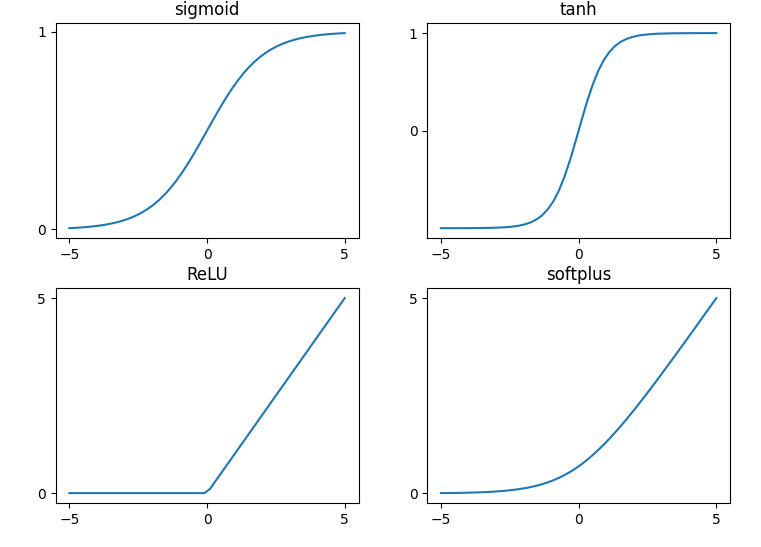
\includegraphics[scale=0.6]{activation_functions.png}
        \caption{Common activation functions, \(\operatorname{sigmoid}\), \(\tanh\), \(\operatorname{ReLU}\), and \(\operatorname{softplus}\), plotted on \([-5, 5]\) for comparison.}
        \label{fig:activation functions}
    \end{figure}
    This simple addition of non-linear activation functions means that a neural network with a single hidden layer containing a finite number of hidden nodes is a universal approximator.
    This means it can approximate any continuous function to arbitrary precision by including more hidden nodes.
    
    \subsection{Different Neural Networks}
    \subsubsection{Deep Learning}
    The term deep learning simply refers to a neural network with many hidden layers.
    A deep learning model has the capacity to deal with high-dimensional data and learn complex features which enable it to perform better on machine learning tasks.
    
    \subsubsection{Convolutional Neural Networks}
    A \gls{cnn} is a neural network with an architecture designed for image processing.
    It uses convolutions between the image and a kernel.
    The image is typically stored as an array of shape \lstinline|(x, y, c)| where \lstinline|x| is the width of the image in pixels, \lstinline|y| is the height of the image in pixels and \lstinline|c| is the number of colour channels, commonly \lstinline|c = 1|, for greyscale images, \lstinline|c=3| for colour images or \lstinline|c = 4| for colour images with opacity levels.
    The way that a convolution works is a smaller kernel is passed over the image and the product of the kernel and the image is calculated at each pixel.
    This gives a single scalar output for each pixel.
    The way that we compute the convolution at a boundary is important.
    Do we replace missing pixels with 0, with 1, with the value of their closest neighbour, with the average of their neighbours, etc. or do we simply drop the edge pixels?
    Whatever we decide the dimensionality is typically reduced if not by dropping edge pixels by reducing multiple colour channels into one.
    The values in the kernel array are the tunable parameters that are represented by the weights of the neural network.
    
    In a \gls{cnn} a convolutional layer is a hidden layer where one or more convolutions are applied at once and then considered together, for example we may consider an image of size \lstinline|(32, 32, 3)| and a kernel of size \lstinline|(5, 5, 3)|.
    After convolution we are left with a feature map of size \lstinline|(28, 28, 1)|, assuming that we simply drop edge pixels.
    Suppose we apply six different kernels to the original image at this point.
    We can feed the six image maps to the next layer of the neural network by considering then as one \lstinline|(28, 28, 6)| array where the colour channels now represent some generalised colour.
    
    As well as convolutional layers \glspl{cnn} also have pooling layers where images are down sampled, for example dropping every other pixel will quarter the size of the image.
    The last few layers of a convolutional neural network typically flatten the image and apply normal neural network layers.
    
    Each convolutional layer picks out different features at different scales and complexities.
    For example the first layer may be very simple and pick out edges and basic patterns.
    The next few layers may pick out more complex textures and colour and the final few layers will pick out objects.
    The network builds up an increasingly complex feature map, all without having to be told what to look for, simply by training the neural network on known images.
    
    \subsubsection{Adversarial Neural Networks}
    An \gls{ann} is uses two neural networks in competition to train each other.
    It is designed for removing bias in data and keeping only the important information from the data.
    The first neural network is a classifier, \(f\), with input \(x\).
    Its output, \(z = f(x)\), is then fed into and adversary network, \(g\), which attempts to measure bias of the classifier.
    If it measures bias then the classifier is penalised.
    The training procedure for a \gls{ann} is as follows:
    \begin{enumerate}
        \item The classifier is pre-trained to minimise the loss function \(L_{\mathrm{clf}}\) with respect to its parameters, \(\vartheta_{\mathrm{clf}}\).
        \item The adversary is then trained on the output of the classifier, without changing the classifier.
        The adversary minimises the loss function \(L_{\mathrm{adv}}\) with respect to its parameters, \(\vartheta_{\mathrm{adv}}\), as well as the parameters of the classifier, \(\vartheta_{\mathrm{adv}}\).
        \item The classifier is then updated with the new loss function \(L_{\mathrm{clf}}' = L_{\mathrm{clf}} - \lambda L_{\mathrm{adv}}\).
        Where \(\lambda > 0\) is a parameter that controls the trade off between the two terms.
        Minimising \(L_{\mathrm{clf}}'\) is finding a balance between minimising \(L_{\mathrm{clf}}\), which corresponds to accurate classification, while maximising \(L_{\mathrm{adv}}\), which corresponds to avoiding bias.
        Increasing \(\lambda\) corresponds to penalising bias more and decreasing \(\lambda\) corresponds to prioritising classification over a lack of bias.
        \item Iterate between steps 2 and 3 until convergence is reached.
    \end{enumerate}
    
    \subsubsection{Auto-Encoders}
    An auto-encoder is used for unsupervised learning.
    It is composed of two parts, an encoder, which takes in data and extracts the important features in some way that allows them to be stored efficiently and a decoder which takes this compressed data and attempts to recover the initial data.
    The hope is that two neural networks can be trained to do this without losing any of the important information.
    The compressed form of the data is called the latent vector.
    It can be visualised as living in some latent space.
    If the encoder does a good job then certain regions of the latent space will correspond to data representing the same thing.
    This means that if we move a little in the latent space then the output of the decoder shouldn't change that much.
    However not all of the latent space corresponds to classified data and therefore if we simply select a random point in the latent space it is unlikely to resemble anything meaningful if we try to decode it.
    
    Auto-encoders are good at encoding and decoding only in the domain they are trained in.
    For example if trained on images of digits and then given an image of a face the encoder will try to encode the face as a digit and since most faces don't look like digits it won't do a very good job and the result of decoding won't look much like a face.
    There is a large reconstruction loss.
    
    We can use this to our benefit in anomaly detection.
    Suppose we have a collection of images and we expect them all to be similar.
    Then we can train an auto-encoder on a set of these images which are similar.
    We can then check for anomalies by using the auto-encoder to encode all of the images and then decoding them.
    We then compare the original image and the decoded image.
    If there are no anomalies in the image then it will be similar to the training data and therefore the reconstruction loss will be small.
    If there is an anomaly then it won't be like the training data and the reconstruction loss will be large.
    Thus by looking for images with a large reconstruction loss we can find anomalous images.
    
    Variational auto-encoders deal with the fact that the latent space isn't categorised everywhere.
    They work similarly to normal auto-encoders but to each input they are trained on they parametrise a Gaussian \gls{pdf} in the latent space.
    This spreads the classification of the point in the latent space over a region.
    This means that points that haven't been classified in the latent space can still be decoded by constructing the latent vector from the \gls{pdf} at that point and decoding it as usual.
    
    One interesting effect of this is we can move around the latent space between two points that represent different properties and see as one morphs into the other.
    We can also use this to create data similar to the data that we start with by sticking close to the classified points but moving around a little.
    
    \subsubsection{Generative Adversarial Networks}
    Generative adversarial networks, similarly to variational auto-encoders, can generate images.
    They do this using a generator, which takes the role of the decoder in a variational auto-encoder, generating images from latent noise, and an adversarial categoriser, known as a discriminator, which attempts to discern which images are real and which are fake.
    Successfully identifying a fake image penalises the generator whereas missing a fake image penalises the discriminator.
    
    While the above description of a generative adversarial network was based on images in theory this model can be used to generate any data and the discriminator can therefore be trained to spot fakes in any data set.
    For example, we may use a generative adversarial network to create fake experimental data which then allows us to use the discriminator to look for anomalies in real experimental data, such as from a particle collider.

    \subsection{Machine Learning in Python}    
    We have seen here the basics of a neural network and how one or more neural networks can work to answer seemingly complicated questions that we may not be able to hard code an answer for.
    The few models we have seen here are only a handful of the existing models and many more exist.
    Often different models work better for different problems and selecting the model that will work best is half of the work.
    Implementing models is often as simple as a call to an imported function.
    There are many modules written for machine learning in python.
    The most common are \lstinline|tensorflow|, and a more user friendly API for it, \lstinline|keras|, \lstinline|scikit-learn|, and \lstinline|pytorch|.
    
    \appendix
    \section{Neural Network Code}
    A \define{perceptron} is another word for what we have been calling a node in section~\ref{sec:machine learning}, another name for a neural network is then a \define{multilayer perceptron}.
    Code implementing a single perceptron which can be trained by back propagation is given here:
    \begin{lstlisting}
    Perceptron.py
    """The class for a single perceptron"""
    
    import numpy as np
    from typing import Iterable, TypeVar
    
    TVec = TypeVar("TVec", Iterable[float], Iterable[int], Iterable[np.float64], Iterable[np.int64], Iterable[np.int32])
    TNum = TypeVar("TNum", float, int)
    
    
    class Perceptron(object):
    """
    A single neuron
    Parameters
    ----------
    inputs : int
    The number of inputs, not including the bias
    bias : float (optional, default bias=1.0)
    The bias term
    """
    
    def __init__(self, inputs: int, bias: TNum = 1.0):
    """
    Create the perceptron object with the specified number of inputs plus 1 for the bias
    
    Parameters
    ----------
    inputs : int
    The number of inputs, not including the bias
    bias : TNum (optional, default bias=1.0)
    The bias term
    
    Returns
    -------
    Perceptron
    The perceptron created
    """
    self.weights = 2 * np.random.random(size=inputs + 1) - 1  # initialise weights as random numbers in [-1, 1)
    self.bias = bias
    self.activation_function = self.sigmoid
    
    def __repr__(self):
    return (f"<Perceptron: inputs = {len(self.weights) - 1}, bias = {self.bias}, weights = {self.weights}, "
    f"at {id(self)}>")
    
    def run(self, x: TVec) -> TVec:
    """
    Run the perceptron
    
    Parameters
    ----------
    x : TVec
    An array of input values
    """
    total = np.dot(np.append(x, self.bias), self.weights)
    return self.activation_function(total)
    
    def set_weights(self, weights_init: TVec):
    """
    Set the weights manually -- useful for testing to insure a consistent starting point
    Parameters
    ----------
    weights_init : TVec
    The values to set the weights to
    """
    if len(weights_init) != len(self.weights):
    raise ValueError(
    f"The length of weights_init, {len(weights_init)}, is not the required {len(self.weights)}")
    self.weights = np.array(weights_init)
    
    def sigmoid(self, x: TVec) -> TVec:
    """
    Sigmoid activation function
    
    Parameters
    ----------
    x : TNum
    
    Returns
    -------
    TVec
    The sigmoid function evaluated at x
    """
    return 1 / (1 + np.exp(-x))
    \end{lstlisting}
    This is easily used to create a multilayer perceptron:
    \begin{lstlisting}
    MultiLayerPerceptron.py
    """Class for the multilayer perceptron"""
    import numpy as np
    from Perceptron import Perceptron, TNum, TVec
    
    
    class MultilayerPerceptron(object):
    """
    A multilayer perceptron class using the Perceptron class
    Parameters
    ----------
    layers :  TVec
    An array containing the number of elements per layer
    bias : TNum (optional, default bias=1.0)
    The bias term, the same bias is used for all neurons
    eta: TNum
    The learing rate
    """
    
    def __init__(self, layers, bias=1.0, eta=0.5):
    """
    Create a multilayer perceptron (MLP)
    Parameters
    ----------
    layers :  TVec
    An array containing the number of elements per layer
    bias : TNum (optional, default bias=1.0)
    The bias term, the same bias is used for all neurons
    eta: TNum
    The learning rate
    Returns
    -------
    MultilayerPerceptron
    A MLP with the specified parameters
    """
    self.layers = np.array(layers, dtype=object)
    self.bias = bias
    self.eta = eta
    self.network = []  # a list of lists of neurons
    self.values = []  # a list of lists of output values
    self.d = []  # a list of error terms
    
    # create network
    for i in range(len(self.layers)):
    self.values.append([])
    self.network.append([])
    self.d.append([])
    self.values[i] = [0.0 for j in range(self.layers[i])]
    self.d[i] = [0.0 for j in range(self.layers[i])]
    if i > 0:  # no neurons in input layer
    for j in range(self.layers[i]):
    self.network[i].append(Perceptron(inputs=self.layers[i - 1], bias=self.bias))
    
    # turn lists into arrays
    self.network = np.array([np.array(x) for x in self.network], dtype=object)
    self.values = np.array([np.array(x) for x in self.values], dtype=object)
    self.values = np.array([np.array(x) for x in self.d], dtype=object)
    
    def set_weights(self, weights_init: TVec):
    """
    Set the weights manually -- useful for testing to insure a consistent starting point
    Parameters
    ----------
    weights_init : TVec
    The values to set the weights to
    """
    for i in range(len(weights_init)):
    for j in range(len(weights_init[i])):
    self.network[i + 1][j].set_weights(weights_init[i][j])
    
    def print_weights(self):
    """
    Print the weights of all neurons
    """
    print()
    for i in range(1, len(self.network)):
    for j in range(self.layers[i]):
    print(f"Layer {i + 1}, Neuron {j}, {self.network[i][j].weights}")
    print()
    
    def run(self, x):
    """
    Run the perceptron
    
    Parameters
    ----------
    x : TVec
    An array of input values
    """
    x = np.array(x, dtype=object)
    self.values[0] = x
    for i in range(1, len(self.network)):
    for j in range(self.layers[i]):
    self.values[i][j] = self.network[i][j].run(self.values[i - 1])
    return self.values[-1]
    
    def back_propagation(self, x: TVec, y: TVec):
    """
    Run a single piece of data, x, and a label, y, with the back propagation algorithm
    Parameters
    ----------
    x : TVec
    The data
    y : TVec
    The correct label for the data
    """
    x = np.array(x, dtype=object)
    y = np.array(y, dtype=object)
    
    # run sample
    output = self.run(x)
    # calculate mean squared error
    n = self.layers[-1]  # n is the number of output neurons
    error = y - output
    mean_squared_error = sum(error ** 2) / n
    
    # calculate output error
    self.d[-1] = output * (1 - output) * error
    
    # calculate the error term of each unit on each layer
    for i in reversed(range(1, len(self.network) - 1)):
    for h in range(len(self.network[i])):
    forward_error = 0.0
    for k in range(self.layers[i + 1]):
    forward_error += self.network[i + 1][k].weights[h] * self.d[i + 1][k]
    self.d[i][h] = self.values[i][h] * (1 - self.values[i][h]) * forward_error
    
    for i in range(1, len(self.network)):
    for j in range(self.layers[i]):
    for k in range(self.layers[i - 1] + 1):
    if k == self.layers[i - 1]:
    delta = self.eta * self.d[i][j] * self.bias
    else:
    delta = self.eta * self.d[i][j] * self.values[i - 1][k]
    self.network[i][j].weights[k] += delta
    
    return mean_squared_error
    \end{lstlisting}
    This can then be used fairly easily, for example in the following a two input, one output multilayer perceptron with a hidden layer of 2 perceptrons is trained to act as an XOR gate.
    This architecture was chosen as a single perceptron can model an AND, OR, or NAND gate and one of each of these can be combined to give an XOR gate, \(A\mathbin{\operatorname{XOR}}B = (A\mathbin{\operatorname{NAND}} B) \mathbin{\operatorname{AND}} (A \mathbin{\operatorname{OR}} B)\).
    \begin{lstlisting}
    XOR_gate.py
    from MultiLayerPerceptron import MultilayerPerceptron
    from logic_gates import test_logic_gate
    
    
    def main():
    mlp = MultilayerPerceptron(layers=[2, 2, 1])
    # uncomment to set the weights to correct values to test error is small
    # and_weights = [10, 10, -15]
    # or_weights = [10, 10, -5]
    # nand_weights = [-10, -10, 15]
    # weights = [[nand_weights, or_weights], [and_weights]]
    # mlp.set_weights(weights)
    
    print("\nTraining Neural Network as an XOR gate...\n")
    epochs = 3000
    for i in range(epochs):
    mean_squared_error = 0.0
    mean_squared_error += mlp.back_propagation([1, 1], [0])
    mean_squared_error += mlp.back_propagation([1, 0], [1])
    mean_squared_error += mlp.back_propagation([0, 1], [1])
    mean_squared_error += mlp.back_propagation([0, 0], [0])
    mean_squared_error /= 4
    if i % 100 == 0:
    print(f"Epoch {i}, current mean squared error: {mean_squared_error}")
    
    test_logic_gate(mlp, "XOR", lambda x, y: int(not (x & y) and (x | y)))
    
    mlp.print_weights()
    
    
    if __name__ == '__main__':
    main()
    \end{lstlisting}
    In this case the possible data to train on is simply the set \(\{(0, 0), (0, 1), (1, 0), (1, 1)\}\) and since this is so small we train on the whole set with the correct labels, \(\{0, 1, 1, 0\}\), respectively.
\end{document}
